% src/slides/source/final.tex

\documentclass[aspectratio=169]{beamer}

% src/slides/source/final/structure/engine.tex
% Adapted from the research presentation template, November 3, 2026.

% Use Carlito through its TeX package so builds do not depend on the user's
% Lua font database being initialized. Use lining numerals throughout the deck
% so digits in body text and section covers align with capital letters.
\usepackage[sfdefault,lining]{carlito}
\pdfmapfile{+carlito.map}
\renewcommand{\familydefault}{\sfdefault}
\usepackage{graphicx}
\usepackage{tikz}
\usepackage{colortbl}

\usetikzlibrary{calc,positioning}

\graphicspath{{assets/}}

\definecolor{MoverNavy}{HTML}{071E47}
\definecolor{MoverSectionNavy}{HTML}{061E4A}
\definecolor{MoverBlue}{HTML}{006CA8}
\definecolor{MoverCyan}{HTML}{0695A1}

\mode<presentation>
{
  \usefonttheme{professionalfonts}

  \setbeamertemplate{navigation symbols}{}
  \setbeamertemplate{headline}{}

  \setbeamercolor{normal text}{
    fg=MoverNavy,
    bg=white
  }

  \setbeamercolor{structure}{
    fg=MoverNavy
  }

  \setbeamercolor{frametitle}{
    fg=white,
    bg=MoverBlue
  }

  \setbeamersize{
    text margin left=0.56cm,
    text margin right=0.10cm
  }
}

\setbeamertemplate{footline}{}
\setbeamertemplate{background}{
  \begin{tikzpicture}[remember picture,overlay]
    \node[anchor=north west,inner sep=0pt]
      at ($(current page.north west)+(0.10cm,-0.08cm)$)
      {
\includegraphics[width=2.65cm]{logos/mover_fubep.png}};

    \node[anchor=south west,inner sep=0pt]
      at ($(current page.south west)+(11.75cm,0.10cm)$)
      {
\includegraphics[height=0.62cm]{logos/unicamp.png}};
    \node[anchor=south west,inner sep=0pt]
      at ($(current page.south west)+(12.62cm,0.10cm)$)
      {
\includegraphics[height=0.62cm]{logos/ufmg.jpg}};
    \node[anchor=south west,inner sep=0pt]
      at ($(current page.south west)+(13.78cm,0.10cm)$)
      {
\includegraphics[width=2.05cm]{logos/eldorado.png}};
  \end{tikzpicture}
}

\setbeamertemplate{frametitle}{
  \nointerlineskip
  \vskip0.50cm

  \hspace*{-0.56cm}%
  \hbox{%
    \begin{beamercolorbox}[
      wd=9.97cm,
      ht=0.76cm,
      dp=0.40cm,
      leftskip=0.25cm,
      rightskip=0.30cm
    ]{frametitle}
      \usebeamerfont{frametitle}
      % Keep title numerals at capital height and on the same baseline (2D, 3D).
      \MoverContentTitleFont
      % Slightly strengthen Carlito Regular; scope the PDF state to the title.
      \pdfliteral direct{2 Tr 0.18 w 1 G}%
      \insertframetitle
      \pdfliteral direct{0 Tr 0 w}%
    \end{beamercolorbox}%
  }

  \vskip-0.22cm

  \begin{tikzpicture}[remember picture,overlay]
    \fill[MoverCyan]
      ($(current page.north west)+(11.47cm,0cm)$)
      rectangle
      ($(current page.north east)+(0cm,-0.37cm)$);

    \node[
      anchor=west,
      text=white,
      inner sep=0pt,
      font=\carlitoTLF\upshape\fontsize{7}{8}\selectfont
    ] at ($(current page.north west)+(11.59cm,-0.185cm)$) {
      \FinalSlideCounter
    };
  \end{tikzpicture}
}

\setbeamerfont{itemize/enumerate body}{
  size=\fontsize{8.5}{10.2}\selectfont
}

\setbeamerfont{itemize/enumerate subbody}{
  size=\fontsize{8.5}{10.2}\selectfont
}

\setbeamertemplate{itemize item}{
  \raise0.25ex
  \hbox{
    \fontsize{6.5}{6.5}\selectfont
    $\bullet$
  }
}

\setbeamertemplate{itemize subitem}{
  \raise0.18ex
  \hbox{
    \fontsize{6.5}{6.5}\selectfont
    $\circ$
  }
}

\setbeamertemplate{itemize subsubitem}{
  \raise0.25ex
  \hbox{
    \fontsize{6.5}{6.5}\selectfont
    $\bullet$
  }
}

\setlength{\leftmargini}{0.49cm}
\setlength{\leftmarginii}{0.79cm}

\newcommand{\MoverListSpacing}{
  \setlength{\itemsep}{0.04cm}
  \setlength{\parskip}{0pt}
  \setlength{\parsep}{0pt}
  \setlength{\topsep}{0pt}
}

\newcommand{\MoverTitleSlide}{
  \begin{frame}
    % Align numerals with capitals in dataset names, 3D, and dates.
    \carlitoLF
    \begin{tikzpicture}[remember picture,overlay]
      \node[
        text=MoverNavy,
        align=center,
        font=\bfseries\fontsize{30}{36}\selectfont
      ] at ($(current page.south west)+(8.00cm,5.91cm)$) {
        \FinalCoverTitleWeight{\MoverPresentationTitle}
      };

      \node[
        anchor=south west,
        text=MoverNavy,
        inner sep=0pt,
        font=\fontsize{8.5}{10.5}\selectfont
      ] at ($(current page.south west)+(0.35cm,0.20cm)$) {
        \MoverPresentationDate
      };

      \node[
        text=MoverNavy,
        align=center,
        text width=11.40cm,
        font=\fontsize{7.6}{9.2}\selectfont
      ] at ($(current page.south west)+(8.00cm,4.17cm)$) {
        \MoverDatasetDescription\\[0.08cm]
        \MoverDatasetReleaseReference
      };

      \node[
        text=MoverNavy,
        align=center,
        text width=8.15cm,
        font=\fontsize{8.8}{10.8}\selectfont
      ] at ($(current page.south west)+(8.08cm,2.14cm)$) {
        \textbf{\underline{\MoverResearcherRole,}}\\
        \MoverResearcherNames
      };
    \end{tikzpicture}
  \end{frame}
}

\newcommand{\MoverThanksSlide}{
  \begin{frame}
    \begin{tikzpicture}[remember picture,overlay]
      \node[
        text=MoverNavy,
        align=center,
        font=\fontsize{34}{40}\selectfont
      ] at ($(current page.south west)+(8.00cm,4.50cm)$) {
        Thank You
      };

      \node[
        text=MoverNavy,
        align=center,
        font=\fontsize{13}{16}\selectfont
      ] at ($(current page.south west)+(8.00cm,3.78cm)$) {
        Questions?
      };
    \end{tikzpicture}
  \end{frame}
}

\newcommand{\MoverSectionPrefix}{}

\AtBeginSection[]
{
  \begin{frame}
    \begin{tikzpicture}[remember picture,overlay]
      \node[
        text=MoverSectionNavy,
        align=center,
        font=\bfseries\fontsize{28}{34}\selectfont
      ] at ($(current page.south west)+(8.00cm,4.50cm)$) {
        \MoverSectionPrefix\insertsection
      };

    \end{tikzpicture}
  \end{frame}
}

\newcommand{\MoverPrompt}[1]{
  \textbf{\underline{#1}}
}

\newcommand{\MoverContentTitleFont}{\carlitoLF\mdseries\upshape\fontsize{18.5}{22}\selectfont}
\newcommand{\MoverContentTitle}[1]{{\MoverContentTitleFont #1}}
\newcommand{\MoverContentTitleLong}[1]{\MoverContentTitle{#1}}
\newcommand{\MoverContentTitleCompact}[1]{\MoverContentTitle{#1}}
\newcommand{\MoverIssueLegendStyle}{\fontsize{7.5}{9.0}\selectfont}
\newenvironment{MoverIssueLegend}{%
  \begin{minipage}[c][5.45cm][c]{\linewidth}%
  \raggedright\MoverIssueLegendStyle
}{%
  \end{minipage}%
}

\newcommand{\MoverSourceCorner}[2][0pt]{
  \smash{%
    \begin{tikzpicture}[remember picture,overlay]
      \node[
        anchor=south east,
        text=MoverNavy,
        fill=white,
        fill opacity=0.88,
        text opacity=1,
        inner sep=1.0pt,
        font=\fontsize{5.8}{6.8}\selectfont
      ] at ($(current page.south east)+(-0.22cm,1.02cm)+(0pt,#1)$) {
        \begin{NoHyper}\textit{Source:} #2\end{NoHyper}
      };
    \end{tikzpicture}%
  }
}

% Generated values come from config/project.toml via build.py.
\input{metadata.generated.tex}

% src/slides/source/final/structure/metadata.tex

% Trim the bold glyph edges slightly without changing font metrics or color.
\newcommand{\FinalCoverTitleWeight}[1]{%
  \pdfliteral direct{2 Tr 0.24 w 1 G}%
  #1%
  \pdfliteral direct{0 Tr 0 w}%
}

\newcommand{\MoverPresentationTitle}{MO809: Final Presentation}
\newcommand{\MoverPresentationDate}{\FinalPresentationDate}
\newcommand{\MoverDatasetDescription}{%
  {\fontsize{19}{24}\selectfont\bfseries
  \FinalCoverTitleWeight{Cooperative Perception with DiscoNet}\\[0.12cm]
  \FinalCoverTitleWeight{Under Perfect Communication}}}
\newcommand{\MoverDatasetReleaseReference}{%
  Learning Distilled Collaboration Graph for Multi-Agent Perception\\[0.08cm]
  Li et al., NeurIPS 2021}
\newcommand{\MoverResearcherRole}{\MakeUppercase{\ProjectAuthor}}
\newcommand{\MoverResearcherNames}{%
  Wellington Lobato, Guilherme Maia,\\
  Allan M. de Souza, Edmundo Madeira}

% src/slides/source/final/structure/layout.tex

% Local compatibility helpers let the final deck reuse the proposal's content
% without editing its frozen cover or changing its rendering.
\usepackage{booktabs}
\usepackage{array}
\usetikzlibrary{arrows.meta}
\DeclareUnicodeCharacter{2192}{\textrightarrow}
\definecolor{MoverDetailBlue}{HTML}{071E47}
\definecolor{MoverPale}{HTML}{EDF5F8}
\hypersetup{colorlinks=true,urlcolor=MoverBlue,linkcolor=MoverNavy}

\newif\ifFinalAppendix
\newcommand{\FinalSlideCounter}{%
  \ifFinalAppendix
    A\insertframenumberinappendix{} / A\insertappendixframenumber
  \else
    \insertframenumber{} / \insertmainframenumber
  \fi
}

\newsavebox{\SlideMeasure}
\newcommand{\SlideBody}[1]{%
  \sbox{\SlideMeasure}{%
    \begin{minipage}{14.80cm}
      \sffamily\fontsize{10.5}{12.8}\selectfont\raggedright
      #1\par
    \end{minipage}}
  \ifdim\dimexpr\ht\SlideMeasure+\dp\SlideMeasure\relax>5.90cm
    \PackageWarning{final-slides}{Slide \insertframenumber\space body exceeds 5.90cm}
  \fi
  \begin{tikzpicture}[remember picture,overlay]
    \node[anchor=north west,inner sep=0pt]
      at ($(current page.north west)+(0.60cm,-1.94cm)$)
      {\usebox{\SlideMeasure}};
  \end{tikzpicture}%
}
\newcommand{\SlideSource}[1]{%
  \begin{tikzpicture}[remember picture,overlay]
    \node[anchor=south west,inner sep=0pt,text width=10.8cm,align=left,
      text=MoverNavy,font=\sffamily\fontsize{7}{9}\selectfont]
      at ($(current page.south west)+(0.60cm,0.39cm)$){\begin{NoHyper}#1\end{NoHyper}};
  \end{tikzpicture}%
}
\newcommand{\FinalPoint}[2]{%
  {\bfseries\fontsize{14}{17}\selectfont #1\par}
  \vspace{0.12cm}#2\par\vspace{0.36cm}
}
\newcommand{\FinalAgendaEntry}[3]{%
  \begin{minipage}[t][1.60cm][t]{6.95cm}
    \makebox[0.62cm][l]{{\fontsize{9}{11}\selectfont #1}}%
    \begin{minipage}[t]{6.23cm}
      \raggedright
      {\fontsize{14}{17}\selectfont\bfseries\strut #2\par}
      \vspace{0.07cm}
      {\fontsize{9.5}{12}\selectfont #3\par}
    \end{minipage}
  \end{minipage}\par
}
\newcommand{\FinalTakeaway}[1]{%
  \begin{tikzpicture}[remember picture,overlay]
    \node[anchor=south west,fill=MoverPale,text=MoverNavy,
      inner sep=5pt,text width=14.1cm,
      font=\sffamily\fontsize{10}{12}\selectfont]
      at ($(current page.south west)+(0.65cm,1.18cm)$) {#1};
  \end{tikzpicture}%
}
\newcommand{\FinalTensorLegend}{%
  {\fontsize{8.5}{10.5}\selectfont
  Tensor shape: $H\times W\times C$\hfill
  $H$ = grid height, $W$ = grid width, $C$ = channels; batch omitted.\par}%
}

% Helpers for slides 2 onward. The frozen cover does not use these commands.
\tikzset{
  visual title/.style={anchor=north west,inner sep=0,align=left,
    text=MoverNavy,font=\sffamily\bfseries\fontsize{14}{17}\selectfont},
  visual label/.style={anchor=north west,inner sep=0,align=left,
    text=MoverDetailBlue,font=\sffamily\bfseries\fontsize{11}{14}\selectfont},
  visual text/.style={anchor=north west,inner sep=0,align=left,
    text=MoverNavy,font=\sffamily\fontsize{11}{14}\selectfont},
  visual small/.style={anchor=north west,inner sep=0,align=left,
    text=MoverDetailBlue,font=\sffamily\fontsize{9}{11}\selectfont},
  visual arrow/.style={-{Stealth[length=2mm]},draw=MoverCyan,line width=1.2pt},
  visual panel/.style={draw=MoverDetailBlue!25,fill=MoverPale,
    rounded corners=3pt,line width=0.5pt}
}
\newenvironment{VisualCanvas}{%
  \begin{tikzpicture}[x=1cm,y=1cm]
    \path[use as bounding box] (0,0) rectangle (14.8,5.75);
}{\end{tikzpicture}}

\newcommand{\VisualTakeaway}[1]{%
  \fill[MoverPale,rounded corners=3pt] (0,0.05) rectangle (14.8,0.85);
  \node[anchor=west,inner sep=0,text width=14.15cm,align=left,
    text=MoverNavy,font=\sffamily\fontsize{11}{14}\selectfont]
    at (0.25,0.45) {#1};
}

\newcommand{\VisualCar}[3]{%
  \begin{scope}[shift={(#1,#2)}]
    \fill[MoverNavy] (-0.44,-0.30) rectangle (-0.23,-0.13);
    \fill[MoverNavy] (0.23,-0.30) rectangle (0.44,-0.13);
    \fill[MoverNavy] (-0.44,0.13) rectangle (-0.23,0.30);
    \fill[MoverNavy] (0.23,0.13) rectangle (0.44,0.30);
    \filldraw[fill=#3,draw=white,line width=0.7pt,rounded corners=3pt]
      (-0.55,-0.23) rectangle (0.55,0.23);
    \fill[white,rounded corners=1pt] (-0.20,-0.16) rectangle (0.18,0.16);
  \end{scope}%
}

% Crop only the top example from each original Figure 5 panel, in the slide
% viewport. The downloaded PNG remains untouched, including author annotations.
\newcommand{\DetectionExample}[2]{%
  \begin{scope}[shift={(#1,0)}]
    \clip (0,1.27) rectangle (4.45,5.17);
    \node[anchor=north west,inner sep=0] at (0,5.17)
      {\includegraphics[width=4.45cm]{assets/papers/disconet/#2}};
  \end{scope}%
}

% src/slides/source/final/structure/minimal-layout.tex

\tikzset{
  final heading/.style={text=MoverNavy,align=center,inner sep=0pt,
    font=\sffamily\bfseries\fontsize{15}{19}\selectfont},
  final caption/.style={text=MoverNavy,align=center,inner sep=0pt,
    font=\sffamily\fontsize{12}{15}\selectfont},
  final statement/.style={text=MoverNavy,align=center,inner sep=0pt,
    font=\sffamily\fontsize{18}{23}\selectfont},
  final icon/.style={draw=MoverNavy,line width=0.9pt,line cap=round,line join=round}
}

% Keep takeaways to a short label, without a paragraph-sized banner.
\renewcommand{\VisualTakeaway}[1]{%
  \node[final caption,text width=14.4cm] at (7.40,0.45) {#1};
}
\renewcommand{\FinalTakeaway}[1]{%
  \begin{tikzpicture}[remember picture,overlay]
    \node[final caption,anchor=south,text width=14.4cm]
      at ($(current page.south west)+(8.00cm,1.20cm)$) {#1};
  \end{tikzpicture}%
}

\newcommand{\FinalCloudIcon}[2]{%
  \begin{scope}[shift={(#1,#2)}]
    \foreach \Point in {(-0.80,-0.35),(-0.62,0.20),(-0.45,0.62),(-0.33,-0.56),
      (-0.15,0.34),(0.02,-0.08),(0.21,0.60),(0.34,-0.42),(0.49,0.10),
      (0.65,0.44),(0.80,-0.19)} {
      \fill[MoverCyan] \Point circle (0.055);
    }
  \end{scope}%
}
\newcommand{\FinalGridIcon}[2]{%
  \begin{scope}[shift={(#1,#2)}]
    \fill[MoverPale] (-0.72,-0.72) rectangle (0.72,0.72);
    \fill[MoverCyan!65] (-0.72,0.24) rectangle (-0.24,0.72);
    \fill[MoverCyan!35] (0,-0.24) rectangle (0.48,0.24);
    \draw[draw=MoverNavy!55,step=0.24,line width=0.5pt]
      (-0.72,-0.72) grid (0.72,0.72);
  \end{scope}%
}
\newcommand{\FinalTableIcon}[2]{%
  \begin{scope}[shift={(#1,#2)}]
    \draw[final icon] (-1,-0.8) rectangle (1,0.8);
    \fill[MoverPale] (-0.98,0.27) rectangle (0.98,0.78);
    \foreach \Row in {-0.27,0.27} {\draw[final icon] (-1,\Row) -- (1,\Row);}
    \foreach \Col in {-0.33,0.33} {\draw[final icon] (\Col,-0.8) -- (\Col,0.8);}
  \end{scope}%
}
\newcommand{\FinalOverlayIcon}[2]{%
  \begin{scope}[shift={(#1,#2)}]
    \draw[draw=MoverNavy!25,line width=0.7pt] (-1.20,-0.9) rectangle (1.20,0.9);
    \draw[draw=MoverCyan,line width=1.7pt,rounded corners=2pt]
      (-0.70,-0.5) rectangle (0.35,0.55);
    \draw[draw=MoverNavy,dashed,line width=0.9pt,rounded corners=2pt]
      (-0.60,-0.45) rectangle (0.45,0.60);
  \end{scope}%
}
\newcommand{\FinalNotebookIcon}[2]{%
  \begin{scope}[shift={(#1,#2)}]
    \draw[final icon,rounded corners=2pt] (-0.82,-1.0) rectangle (0.82,1.0);
    \draw[draw=MoverCyan,line width=1pt] (-0.52,0.62) -- (0.52,0.62);
    \draw[final icon] (-0.18,0.28) -- (-0.45,0.04) -- (-0.18,-0.20);
    \draw[final icon] (0.18,0.28) -- (0.45,0.04) -- (0.18,-0.20);
    \draw[final icon] (-0.50,-0.61) -- (0.50,-0.61);
  \end{scope}%
}
\newcommand{\FinalModelIcon}[2]{%
  \begin{scope}[shift={(#1,#2)}]
    \foreach \LeftY in {-0.38,0.38} {
      \foreach \RightY in {-0.38,0.38} {
        \draw[draw=MoverNavy!35,line width=0.7pt] (-0.9,\LeftY) -- (0,\RightY);
        \draw[draw=MoverNavy!35,line width=0.7pt] (0,\LeftY) -- (0.9,\RightY);
      }
    }
    \foreach \Col in {-0.9,0,0.9} {
      \foreach \Row in {-0.38,0.38} {
        \filldraw[fill=white,draw=MoverCyan,line width=1pt] (\Col,\Row) circle (0.13);
      }
    }
  \end{scope}%
}
\renewcommand{\FinalTensorLegend}{%
  {\centering\fontsize{9}{11}\selectfont
  $H$ = Height\quad $W$ = Width\quad $C$ = Channels\par}%
}

% Preserve PDF text, plots, code, and figure resolution in the hand-in appendix.
% Snapshot inputs and complete source-page coverage are in assets/appendix/.

\newcommand{\FinalAppendixCounter}{%
  \fill[MoverCyan]
    ($(current page.north west)+(11.47cm,0cm)$) rectangle
    ($(current page.north east)+(0cm,-0.37cm)$);
  \node[anchor=west,text=white,inner sep=0pt,
    font=\carlitoTLF\upshape\fontsize{7}{8}\selectfont]
    at ($(current page.north west)+(11.59cm,-0.185cm)$)
    {\FinalSlideCounter};
}

\newcommand{\FinalAppendixDivider}[4]{%
  \section{#1. #2}
  \begin{frame}[label=appendix-#3]
    \begin{tikzpicture}[remember picture,overlay]
      \node[text=MoverSectionNavy,align=center,inner sep=0pt,
        font=\bfseries\fontsize{14}{18}\selectfont]
        at ($(current page.south west)+(8.00cm,5.55cm)$) {Appendix #1};
      \node[text=MoverSectionNavy,align=center,text width=14.6cm,inner sep=0pt,
        font=\bfseries\fontsize{26}{32}\selectfont]
        at ($(current page.south west)+(8.00cm,4.45cm)$) {#2};
      \node[text=MoverNavy,align=center,text width=12.5cm,inner sep=0pt,
        font=\fontsize{11}{14}\selectfont]
        at ($(current page.south west)+(8.00cm,2.95cm)$) {#4};
      \FinalAppendixCounter
    \end{tikzpicture}
  \end{frame}
}

\newcommand{\FinalWeeklyAppendixPage}[2]{%
  \begingroup
  \setbeamertemplate{background}{}
  \begin{frame}[plain,label=appendix-weekly-#1]
    \pdfbookmark[2]{Weekly #1: #2}{appendix-weekly-bookmark-#1}
    \begin{tikzpicture}[remember picture,overlay]
      \node[anchor=south west,inner sep=0pt] at (current page.south west)
        {\includegraphics[page=#1,width=\paperwidth,height=\paperheight]
          {appendix/weekly.pdf}};
      \FinalAppendixCounter
    \end{tikzpicture}
  \end{frame}
  \endgroup
}

\newcommand{\FinalExperimentAppendixPage}[2]{%
  \begingroup
  \setbeamertemplate{background}{}
  \begin{frame}[plain,label=appendix-experiments-#1]
    \pdfbookmark[2]{Report #1: #2}{appendix-experiments-bookmark-#1}
    \begin{tikzpicture}[remember picture,overlay]
      \node[anchor=south west,inner sep=0pt] at (current page.south west)
        {\includegraphics[page=#1,width=\paperwidth,height=\paperheight]
          {appendix/disconet-experiments.pdf}};
      \FinalAppendixCounter
      % The source report's bottom-right page number is navigation only.
      \fill[white] ($(current page.south east)+(-2.20cm,0.12cm)$) rectangle
        ($(current page.south east)+(-0.40cm,0.55cm)$);
      \node[anchor=south east,text=MoverNavy,inner sep=0pt,
        font=\fontsize{5}{6}\selectfont]
        at ($(current page.south east)+(-0.60cm,0.24cm)$)
        {DiscoNet Report, p.\,#1};
    \end{tikzpicture}
  \end{frame}
  \endgroup
}


\title{MO809 Final Presentation: \ProjectTitle}
\author{\ProjectAuthor}
\hypersetup{pdftitle={MO809 Final Presentation: \ProjectTitle},
  pdfauthor={\ProjectAuthor},pdfsubject={MO809 final project presentation}}

% The delivered talk keeps its original 1--29 numbering. Supplementary pages
% use the appendix counters defined in final/structure/layout.tex.

\begin{document}

\MoverTitleSlide
% src/slides/source/final/sections/00_agenda.tex

\begin{frame}{Agenda}
  \SlideBody{\begin{VisualCanvas}
    \foreach \Number/\Topic [count=\Index from 0] in {
      01/Motivation,
      02/Problem,
      03/Project Objective,
      04/Project Development,
      05/Evaluation,
      06/Results} {
      \pgfmathsetmacro{\RowY}{5.05-0.84*\Index}
      \node[anchor=west,inner sep=0pt,text=MoverNavy,
        font=\sffamily\fontsize{9}{11}\selectfont]
        at (0.10,\RowY) {\Number};
      \node[anchor=west,inner sep=0pt,text=MoverNavy,
        font=\sffamily\bfseries\fontsize{14}{17}\selectfont]
        at (0.82,\RowY) {\Topic};
    }
  \end{VisualCanvas}}
\end{frame}


\section{Motivation}
% src/slides/source/final/core/01_motivation.tex

\begin{frame}{Cooperative Perception}
  \SlideBody{\centering
    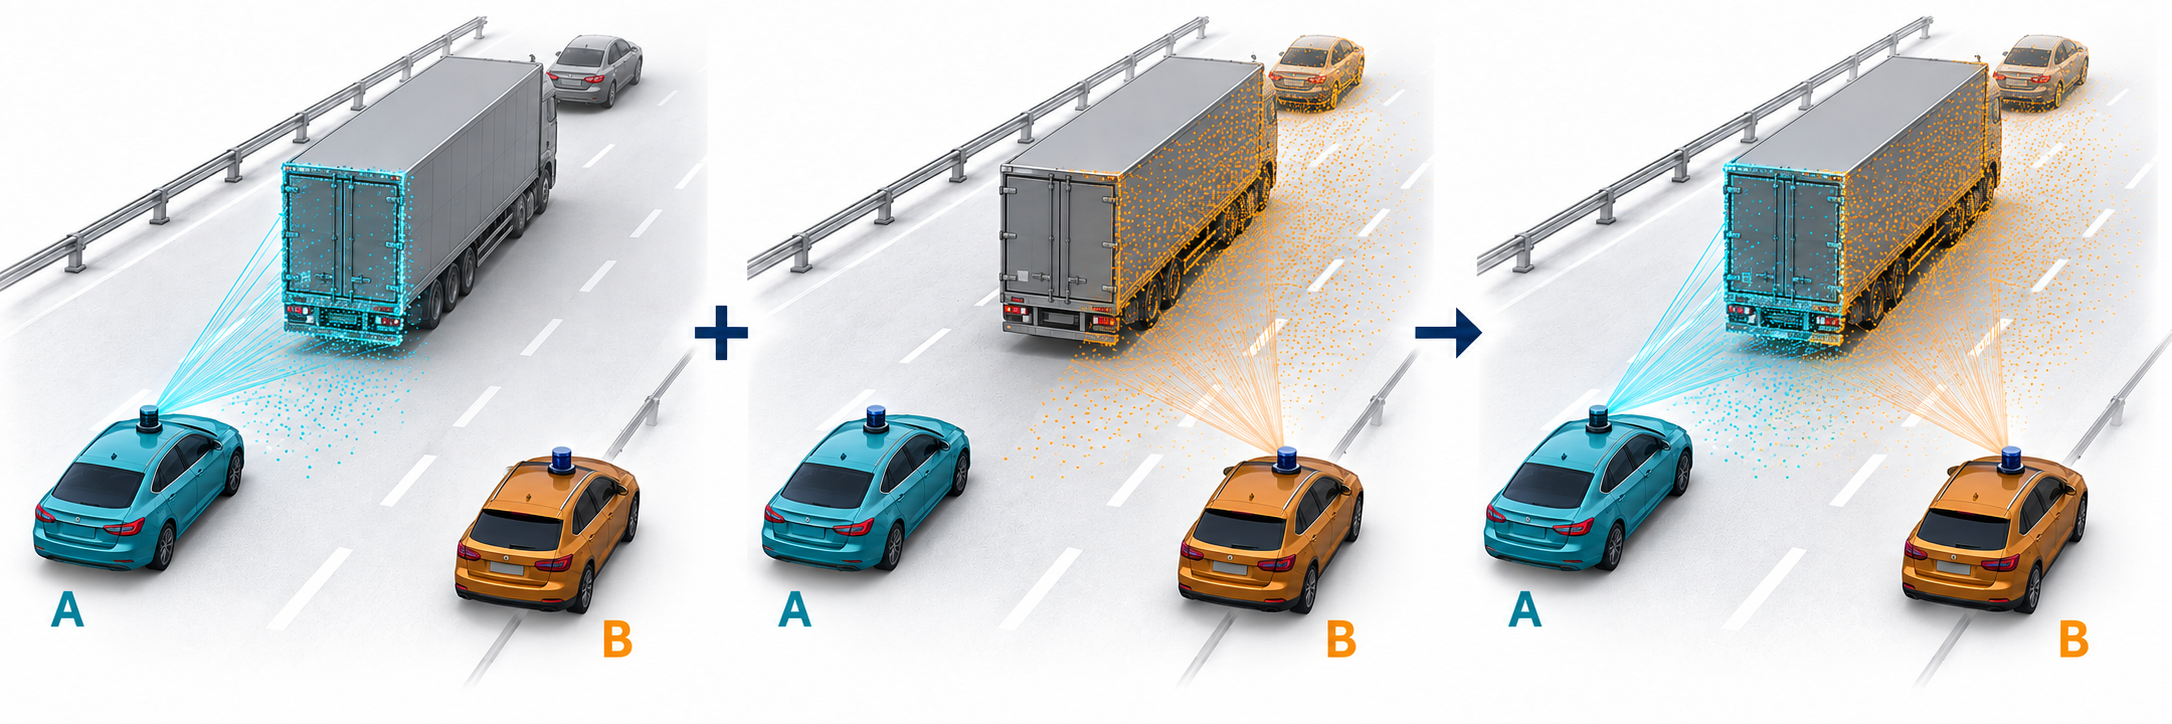
\includegraphics[width=14.65cm,height=5.05cm,keepaspectratio]{assets/illustrations/lidar-cooperation-v2.png}\par
  }
  \FinalTakeaway{Seeing Beyond One View}
  \SlideSource{Source: AI generated illustration.}
\end{frame}

% src/slides/source/final/core/01b_collaboration_strategies.tex

\begin{frame}{Collaboration Strategies}
  \SlideBody{\begin{VisualCanvas}
    \node[final heading] at (3.4,5.45) {Early Fusion};
    \node[final heading] at (7.4,5.45) {Intermediate Fusion};
    \node[final heading] at (11.4,5.45) {Late Fusion};
    \draw[draw=MoverCyan,line width=1.5pt] (5.8,5.10) -- (9.0,5.10);
    \node[inner sep=0pt] at (7.4,3.10)
      {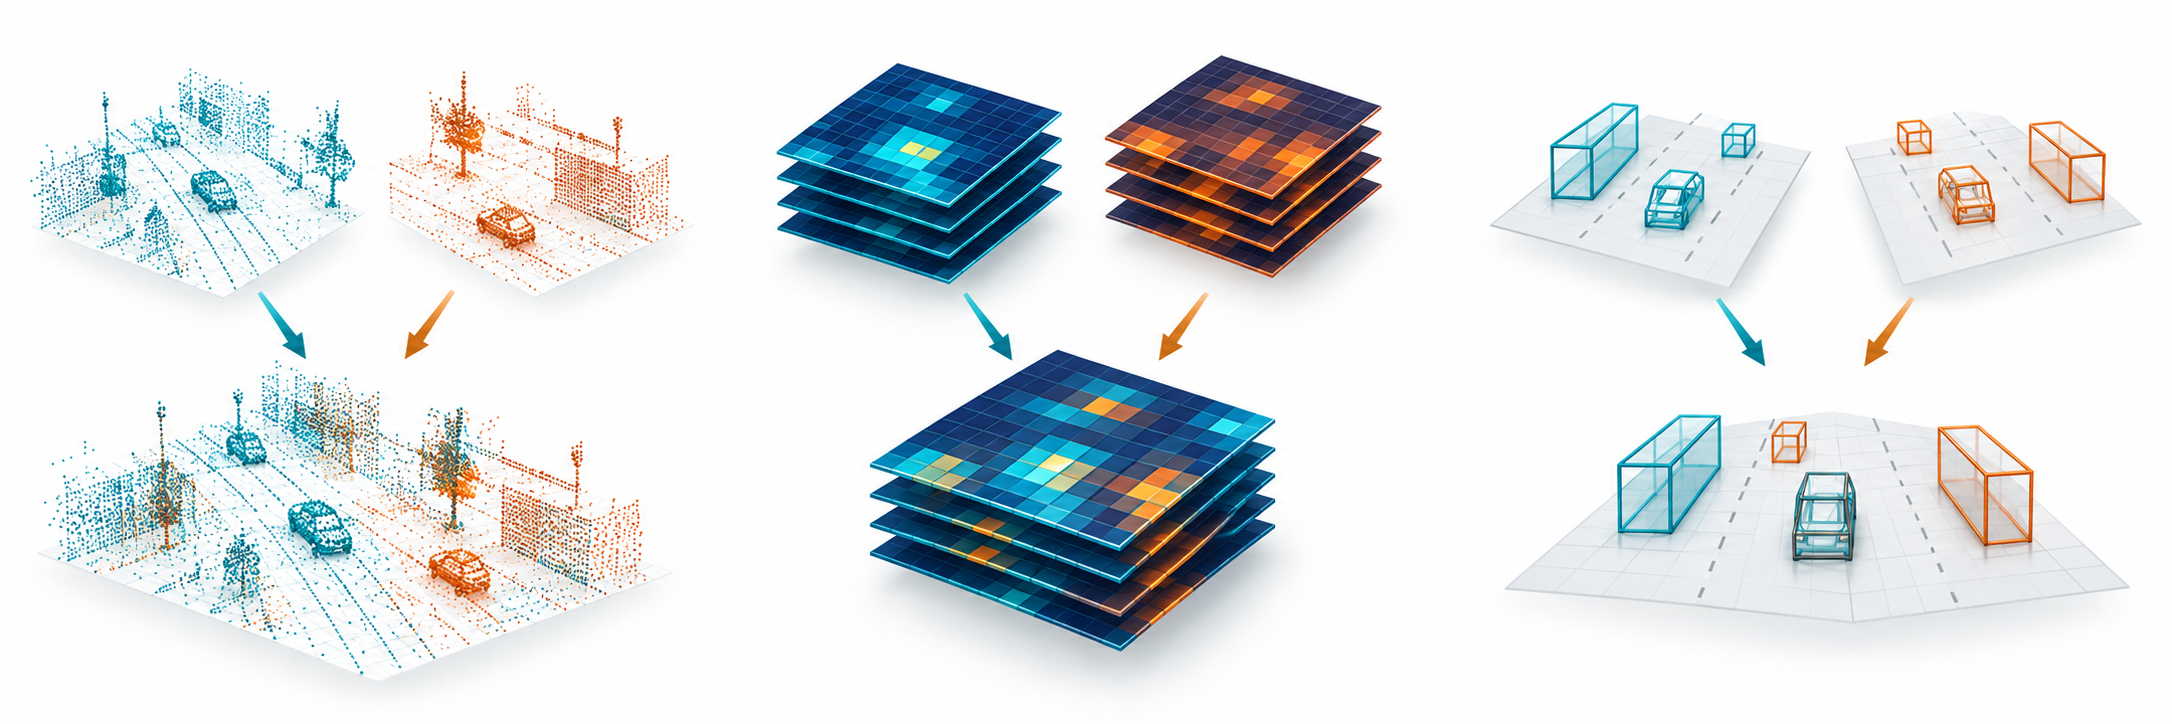
\includegraphics[width=12.0cm]{assets/illustrations/fusion-strategies.png}};
    \node[final caption] at (3.4,0.95) {Raw Points};
    \node[final caption] at (7.4,0.95) {Learned Features};
    \node[final caption] at (11.4,0.95) {Boxes + Scores};
    \node[visual small,anchor=center] at (3.4,0.52) {Before Encoding};
    \node[visual small,anchor=center] at (7.4,0.52) {Before Detection};
    \node[visual small,anchor=center] at (11.4,0.52) {After Detection};
  \end{VisualCanvas}}
  \SlideSource{Source: AI generated illustrations.}
\end{frame}

\section{Problem}
% src/slides/source/final/core/02_problem.tex

\begin{frame}{Problem}
  \SlideBody{\begin{VisualCanvas}
    \node[final statement,text width=14.4cm,
      font=\sffamily\fontsize{16}{20}\selectfont] at (7.4,5.28)
      {Can a Holistic Early-Fusion Model Be Compressed\\
      While Preserving Detection Accuracy?};
    \begin{scope}[yshift=-0.20cm,overlay]
      \node[inner sep=0pt] at (7.4,2.70)
        {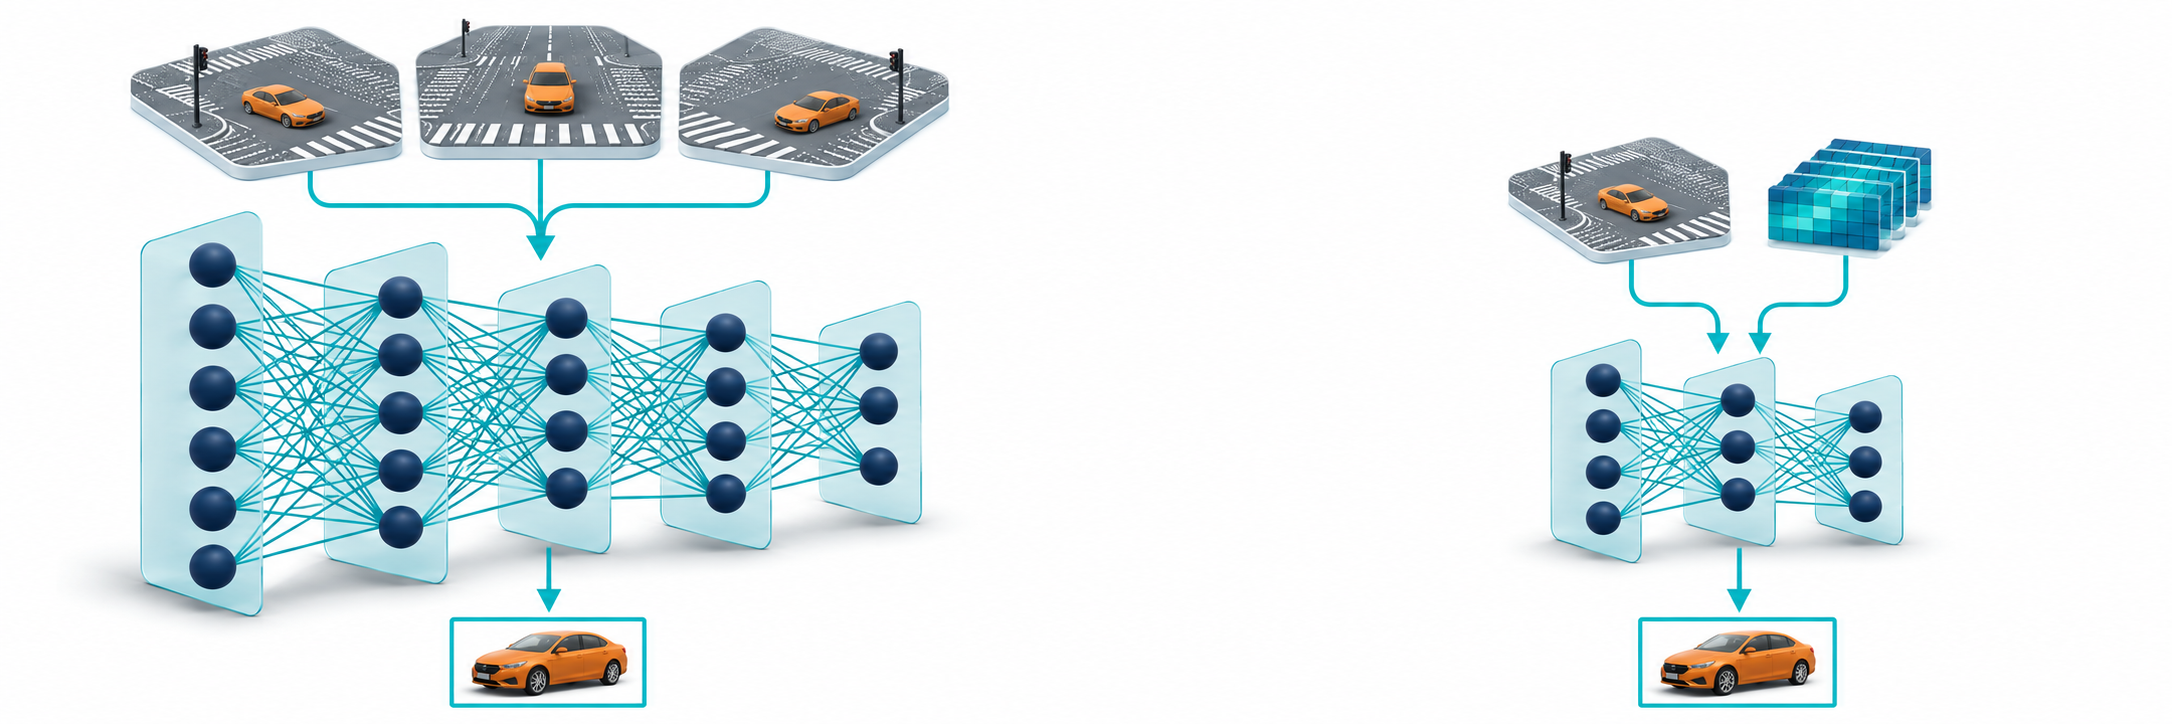
\includegraphics[width=11.7cm]{assets/illustrations/problem/problem-model-distillation-imagegen-v4.png}};
      \node[final heading] at (4.5,0.55) {Teacher};
      \node[final heading] at (11.0,0.55) {Student};
      \node[visual small,anchor=center] at (4.5,0.14) {Holistic View};
      \node[visual small,anchor=center] at (11.0,0.14) {Local + Shared Features};
      \draw[visual arrow,dashed] (6.90,2.70) --
        node[above,align=center,text=MoverNavy,font=\fontsize{9}{11}\selectfont]
          {Distillation\\Training Only} (9.90,2.70);
    \end{scope}
  \end{VisualCanvas}}
  \SlideSource{Source: AI generated illustrations.}
\end{frame}

% src/slides/source/final/core/02a_paper_strategy.tex

\begin{frame}{DiscoNet Collaboration Strategy}
  \SlideBody{\begin{VisualCanvas}
    \node[inner sep=0pt] at (7.4,2.875)
      {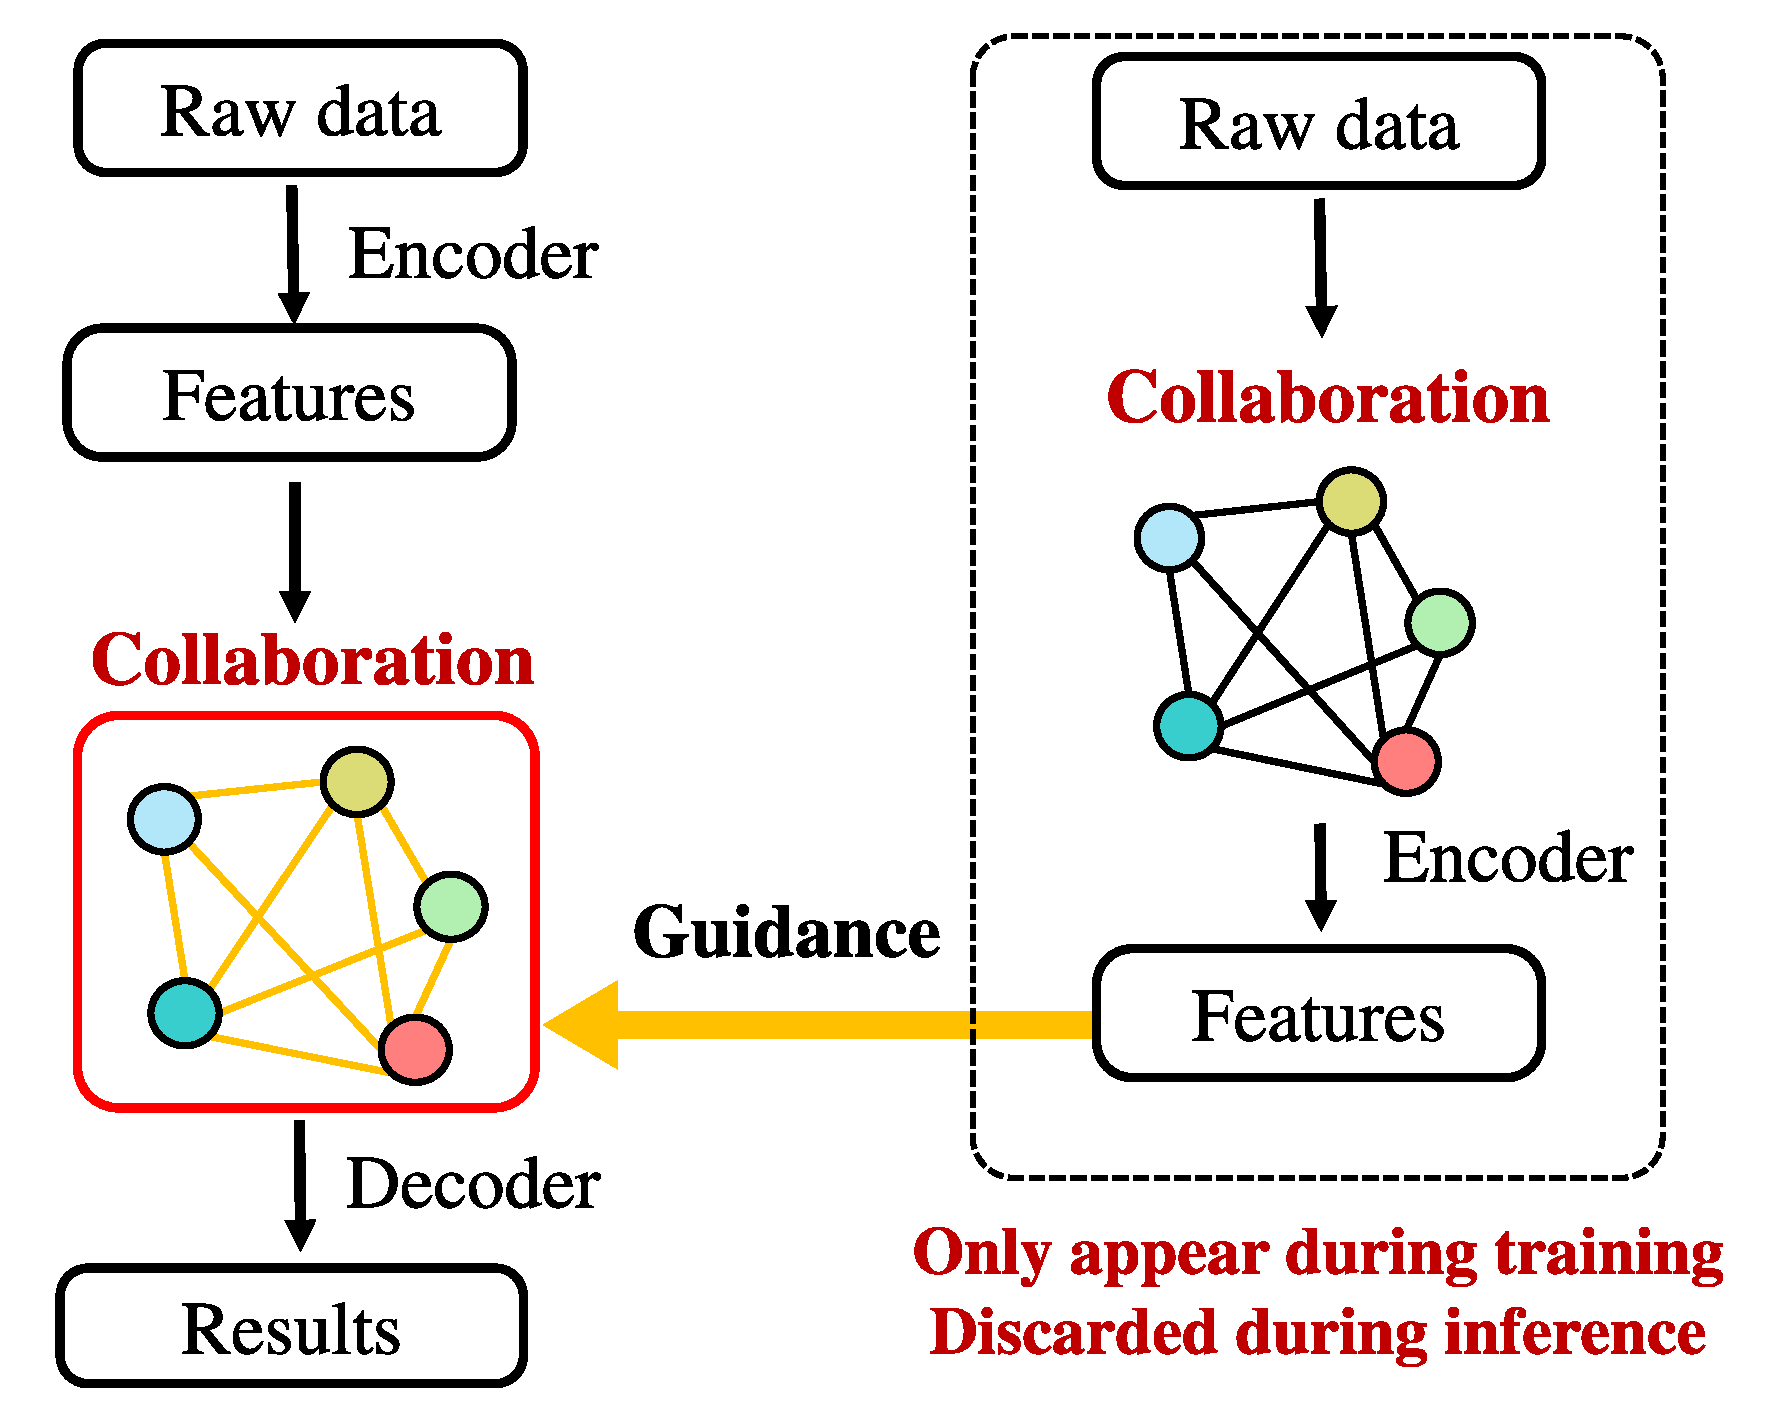
\includegraphics[width=7.0cm,height=5.60cm,keepaspectratio]{assets/papers/disconet/fig1_ours.pdf}};
    \node[final heading] at (2.0,3.65) {Student};
    \node[final caption,text width=3.4cm] at (2.0,2.80)
      {Intermediate\\Collaboration};
    \node[final heading] at (12.8,3.65) {Teacher};
    \node[final caption,text width=3.4cm] at (12.8,2.80)
      {Early\\Collaboration};
  \end{VisualCanvas}}
  \SlideSource{Source: Li et al., DiscoNet, Figure 1(c).}
\end{frame}

% src/slides/source/final/core/02b_paper_architecture.tex

\begin{frame}{DiscoNet Architecture}
  \SlideBody{\begin{VisualCanvas}
    \node[inner sep=0pt] at (7.4,2.875)
      {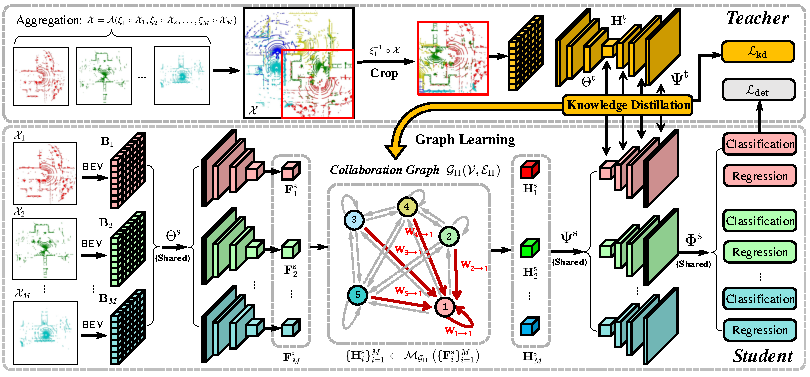
\includegraphics[width=14.4cm,height=5.75cm,keepaspectratio]{assets/papers/disconet/fig2_overview.pdf}};
  \end{VisualCanvas}}
  \SlideSource{Source: Li et al., DiscoNet, Figure 2.}
\end{frame}

\section{Project Objective}
% src/slides/source/final/core/03_objective.tex

\begin{frame}{Project Objective}
  \SlideBody{\begin{VisualCanvas}
    \node[final statement,text width=14.4cm,
      font=\sffamily\fontsize{16}{20}\selectfont] at (7.4,5.15)
      {Evaluate DiscoNet's Detection Quality and Scalability\\
      under Perfect Communication};
    \node[inner sep=0pt] at (2.4,3.32)
      {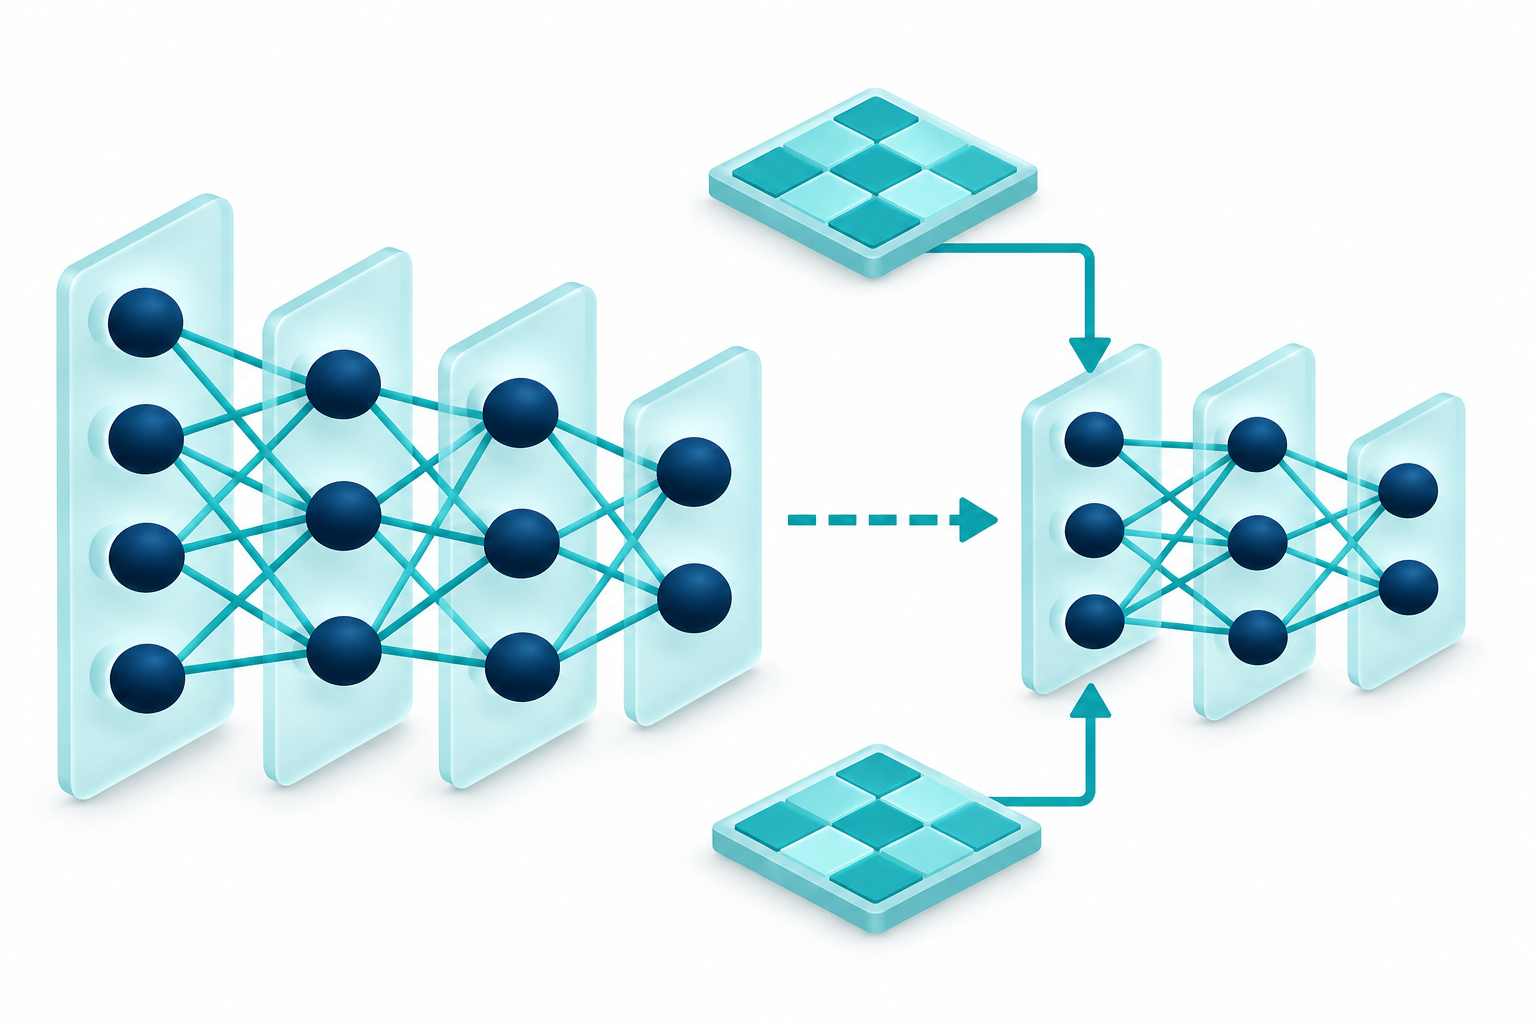
\includegraphics[width=4.0cm,height=2.45cm,keepaspectratio]{assets/illustrations/objective/understand-imagegen-v1.png}};
    \node[inner sep=0pt] at (7.4,3.32)
      {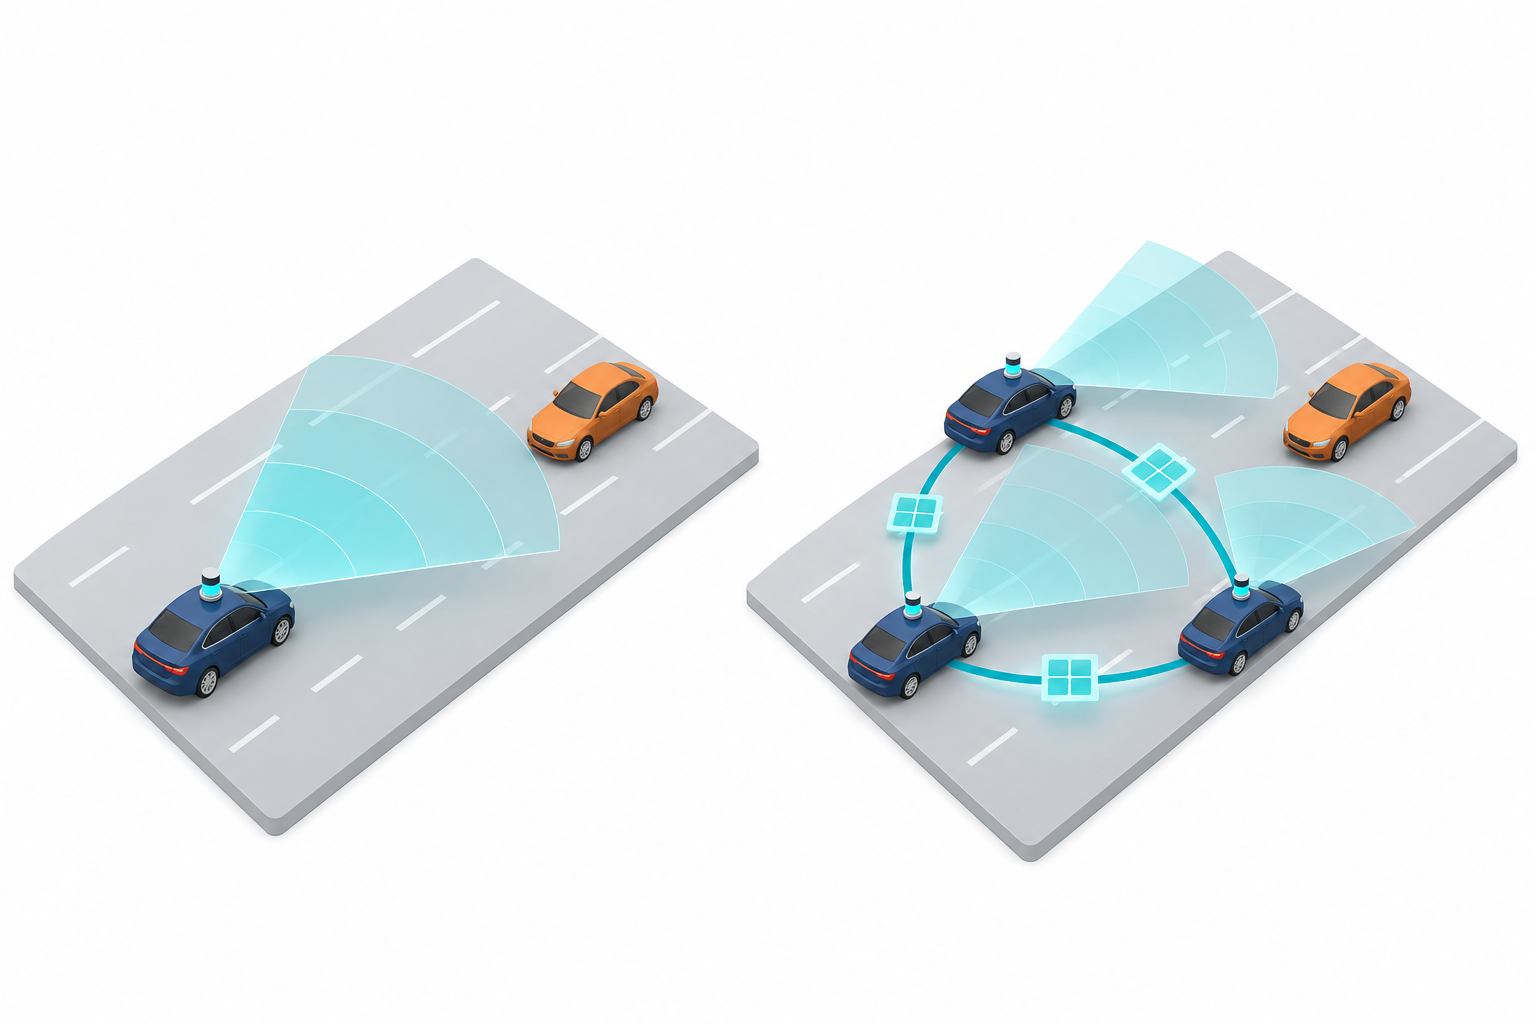
\includegraphics[width=4.0cm,height=2.45cm,keepaspectratio]{assets/illustrations/objective/compare-imagegen-v1.png}};
    \node[inner sep=0pt] at (12.4,3.32)
      {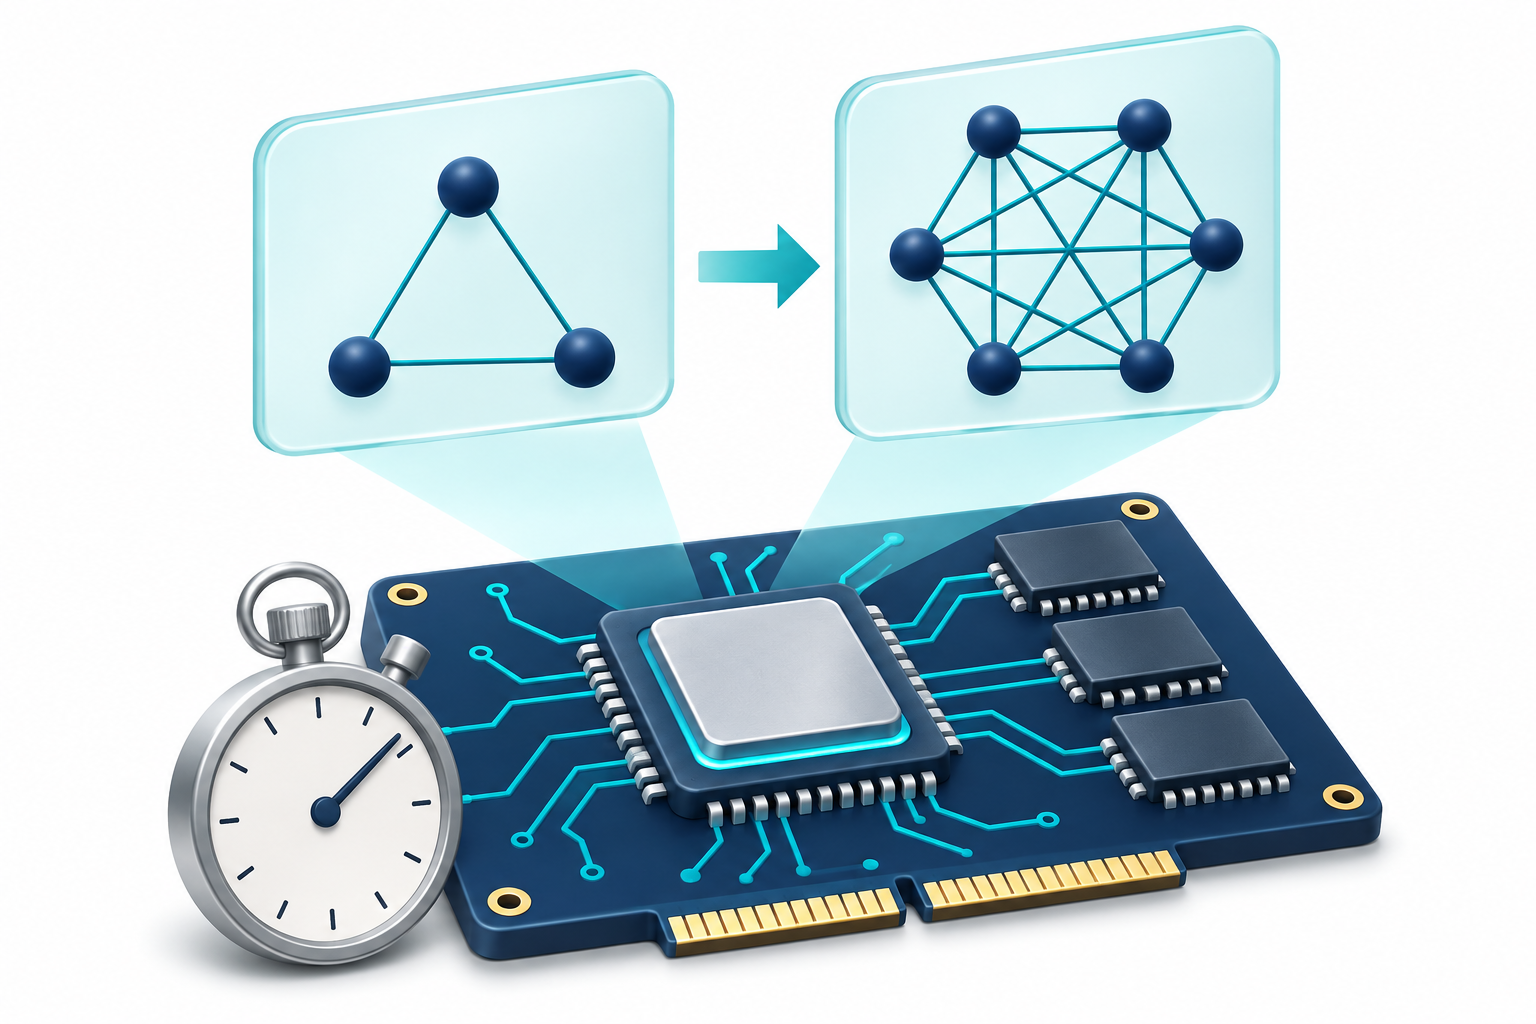
\includegraphics[width=4.0cm,height=2.45cm,keepaspectratio]{assets/illustrations/objective/benchmark-imagegen-v1.png}};
    \draw[visual arrow] (4.55,3.32) -- (5.25,3.32);
    \draw[visual arrow] (9.55,3.32) -- (10.25,3.32);
    \node[final heading] at (2.4,1.80) {Understand};
    \node[final heading] at (7.4,1.80) {Compare};
    \node[final heading] at (12.4,1.80) {Benchmark};
    \node[final caption,text width=4.4cm,
      font=\fontsize{11}{14}\selectfont] at (2.4,0.98)
      {Teacher--Student Pipeline\\and Feature Fusion};
    \node[final caption,text width=4.4cm,
      font=\fontsize{11}{14}\selectfont] at (7.4,0.98)
      {Individual vs.\\Cooperative Detection};
    \node[final caption,text width=4.4cm,
      font=\fontsize{11}{14}\selectfont] at (12.4,0.98)
      {Accuracy and Cost\\as $n$ Increases};
    \node[visual small,anchor=center] at (7.4,0.15)
      {$n$ = Number of Cooperating Agents};
  \end{VisualCanvas}}
  \SlideSource{Source: AI generated illustrations.}
\end{frame}

% src/slides/source/final/core/03b_scaling_proposal.tex

\begin{frame}{Our Proposal: Accuracy and Scale}
  \SlideBody{\begin{VisualCanvas}
    \node[final statement,font=\fontsize{16}{20}\selectfont]
      at (7.4,5.35) {Benchmark the Limits of Full Collaboration};

    % Each drawn connection represents both directed peer interactions.
    % Self-pairs are included in attention, but omitted from these glyphs.
    \foreach \AgentCount/\CenterX/\PairCount in {2/2.5/2,4/7.4/12,8/12.3/56} {
      \node[final heading] at (\CenterX,4.65) {$n=\AgentCount$};
      \foreach \Agent in {1,...,\AgentCount} {
        \pgfmathsetmacro{\Angle}{90+360*(\Agent-1)/\AgentCount}
        \coordinate (agent-\AgentCount-\Agent) at
          ({\CenterX+1.10*cos(\Angle)},{3.00+1.10*sin(\Angle)});
      }
      \foreach \Sender in {1,...,\AgentCount} {
        \foreach \Receiver in {1,...,\AgentCount} {
          \ifnum\Sender<\Receiver
            \draw[{Stealth[length=1.0mm]}-{Stealth[length=1.0mm]},
              draw=MoverNavy!40,line width=0.5pt,shorten <=3pt,shorten >=3pt]
              (agent-\AgentCount-\Sender) -- (agent-\AgentCount-\Receiver);
          \fi
        }
      }
      \foreach \Agent in {1,...,\AgentCount} {
        \filldraw[fill=MoverNavy,draw=MoverCyan,line width=0.8pt]
          (agent-\AgentCount-\Agent) circle (0.10cm);
      }
      \node[final caption,text width=4.4cm] at (\CenterX,1.35)
        {\PairCount\ Directed Peer Pairs};
    }
    \draw[visual arrow] (3.95,3.00) -- (5.95,3.00);
    \draw[visual arrow] (8.85,3.00) -- (10.85,3.00);
    % For fixed feature dimensions, pairwise work is quadratic in agent count.
    \node[final caption] at (7.4,0.78)
      {Quadratic Pairwise Work: $n(n-1)=\mathcal{O}(n^2)$};
    \node[final caption] at (7.4,0.20)
      {Measure AP and Time Inference};
  \end{VisualCanvas}}
\end{frame}

\begin{frame}{Local vs. Cooperative Detection}
  \SlideBody{\begin{VisualCanvas}
    % Trim only blank outer margins; keep every plotted mark and legend.
    \node[inner sep=0pt] at (7.4,2.875)
      {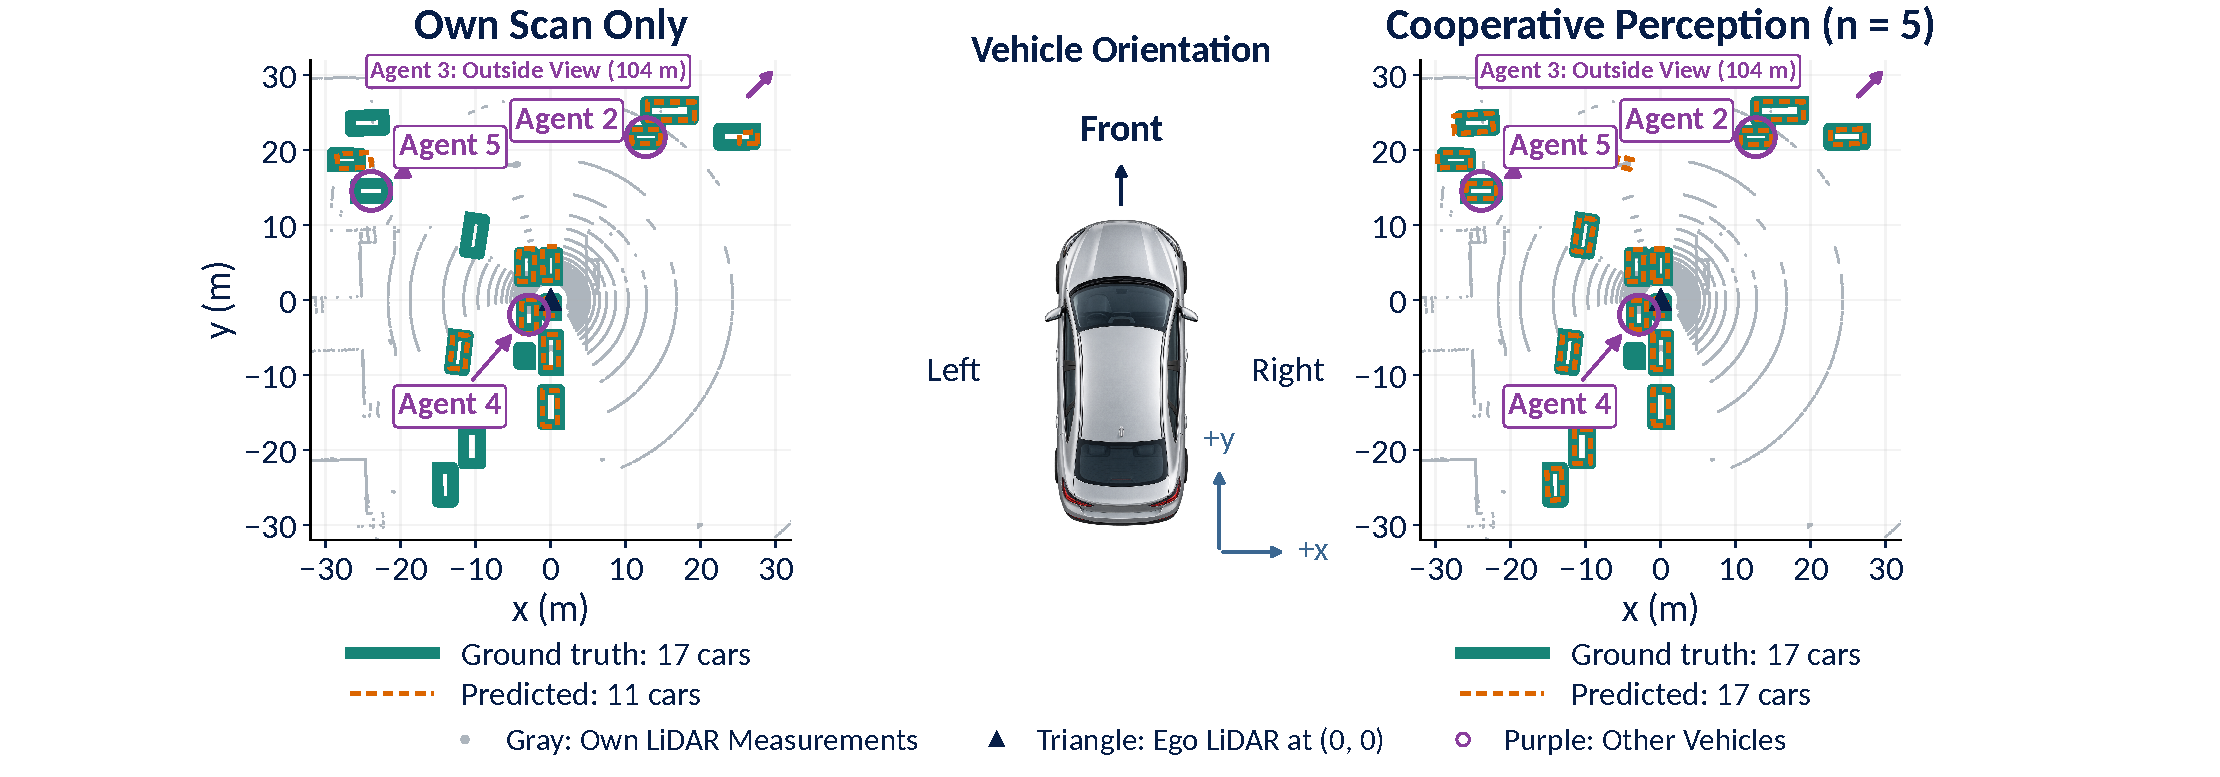
\includegraphics[trim=90bp 5bp 130bp 0bp,clip,
        width=14.8cm,height=5.75cm,keepaspectratio]{assets/experiments/w45-2026-11-04/example-detections-v1.pdf}};
  \end{VisualCanvas}}
  \begin{tikzpicture}[remember picture,overlay]
    \node[visual small,anchor=center]
      at ($(current page.south west)+(8.00cm,0.98cm)$)
      {One Example: Scene 5, Raw Frame 000066; Ego Vehicle 1};
  \end{tikzpicture}
  \SlideSource{Source: AI generated illustrations.}
\end{frame}

\section{Project Development}
% src/slides/source/final/core/04_development.tex

\begin{frame}{Project Development}
  \SlideBody{\begin{VisualCanvas}
    \node[final heading] at (2.4,5.0) {Data};
    \node[final heading] at (7.4,5.0) {Models};
    \node[final heading] at (12.4,5.0) {Evidence};
    \node[inner sep=0pt] at (2.4,3.28)
      {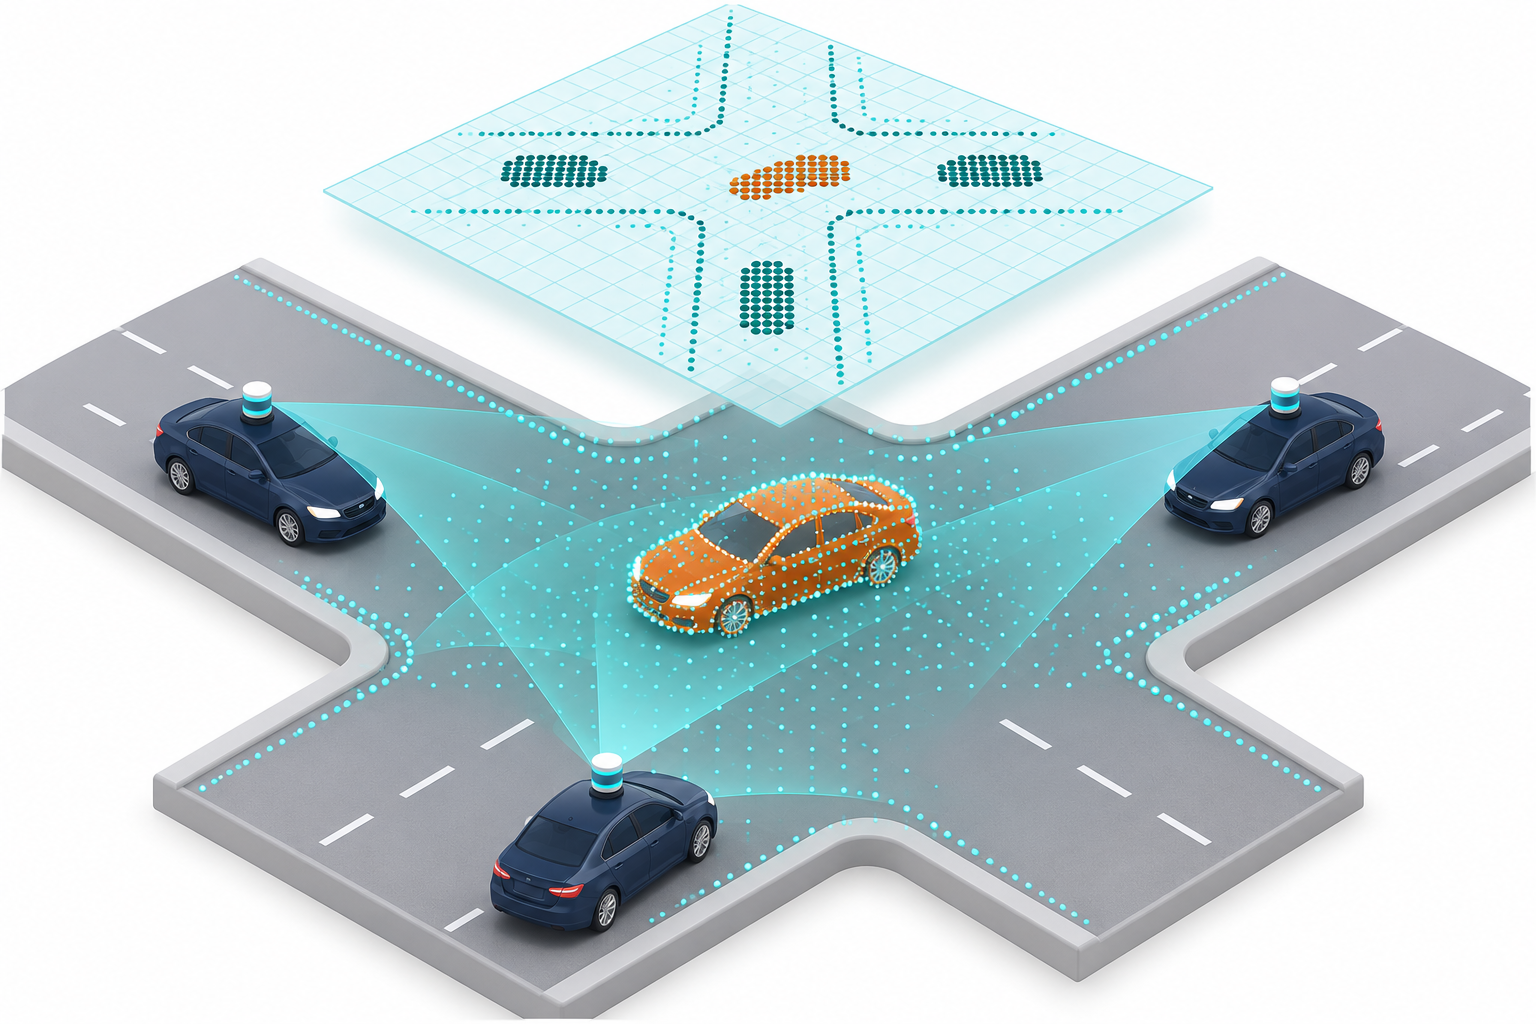
\includegraphics[width=4.0cm,height=2.65cm,keepaspectratio]{assets/illustrations/development/data-imagegen-v1.png}};
    \node[inner sep=0pt] at (7.4,3.28)
      {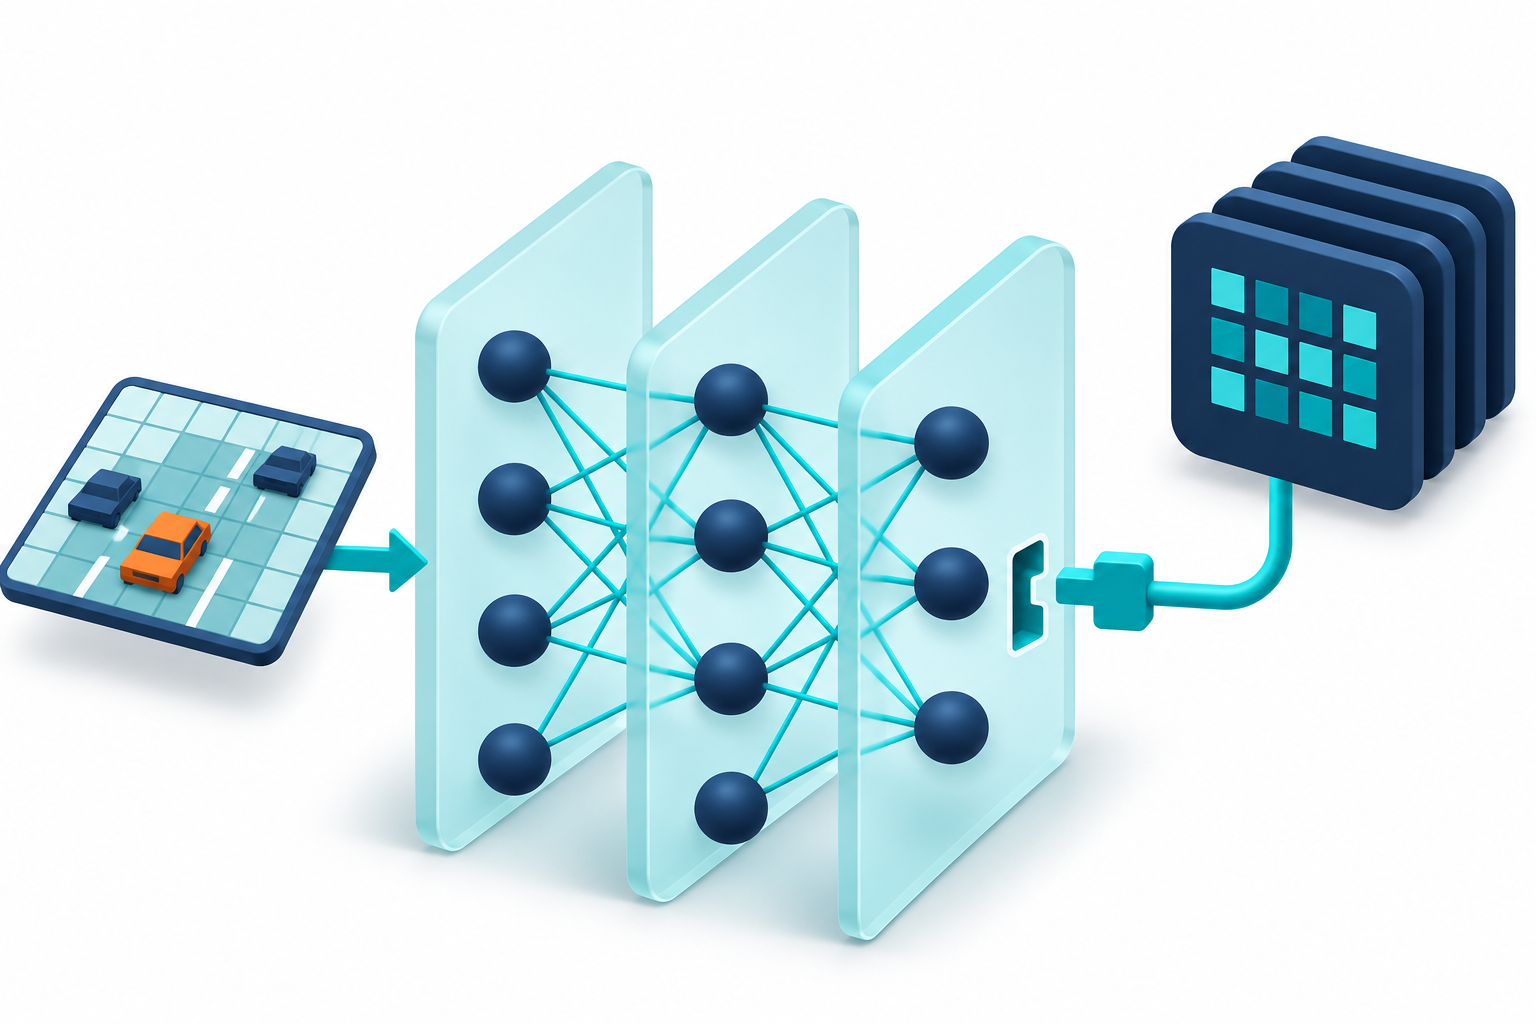
\includegraphics[width=4.0cm,height=2.65cm,keepaspectratio]{assets/illustrations/development/models-imagegen-v1.png}};
    \node[inner sep=0pt] at (12.4,3.28)
      {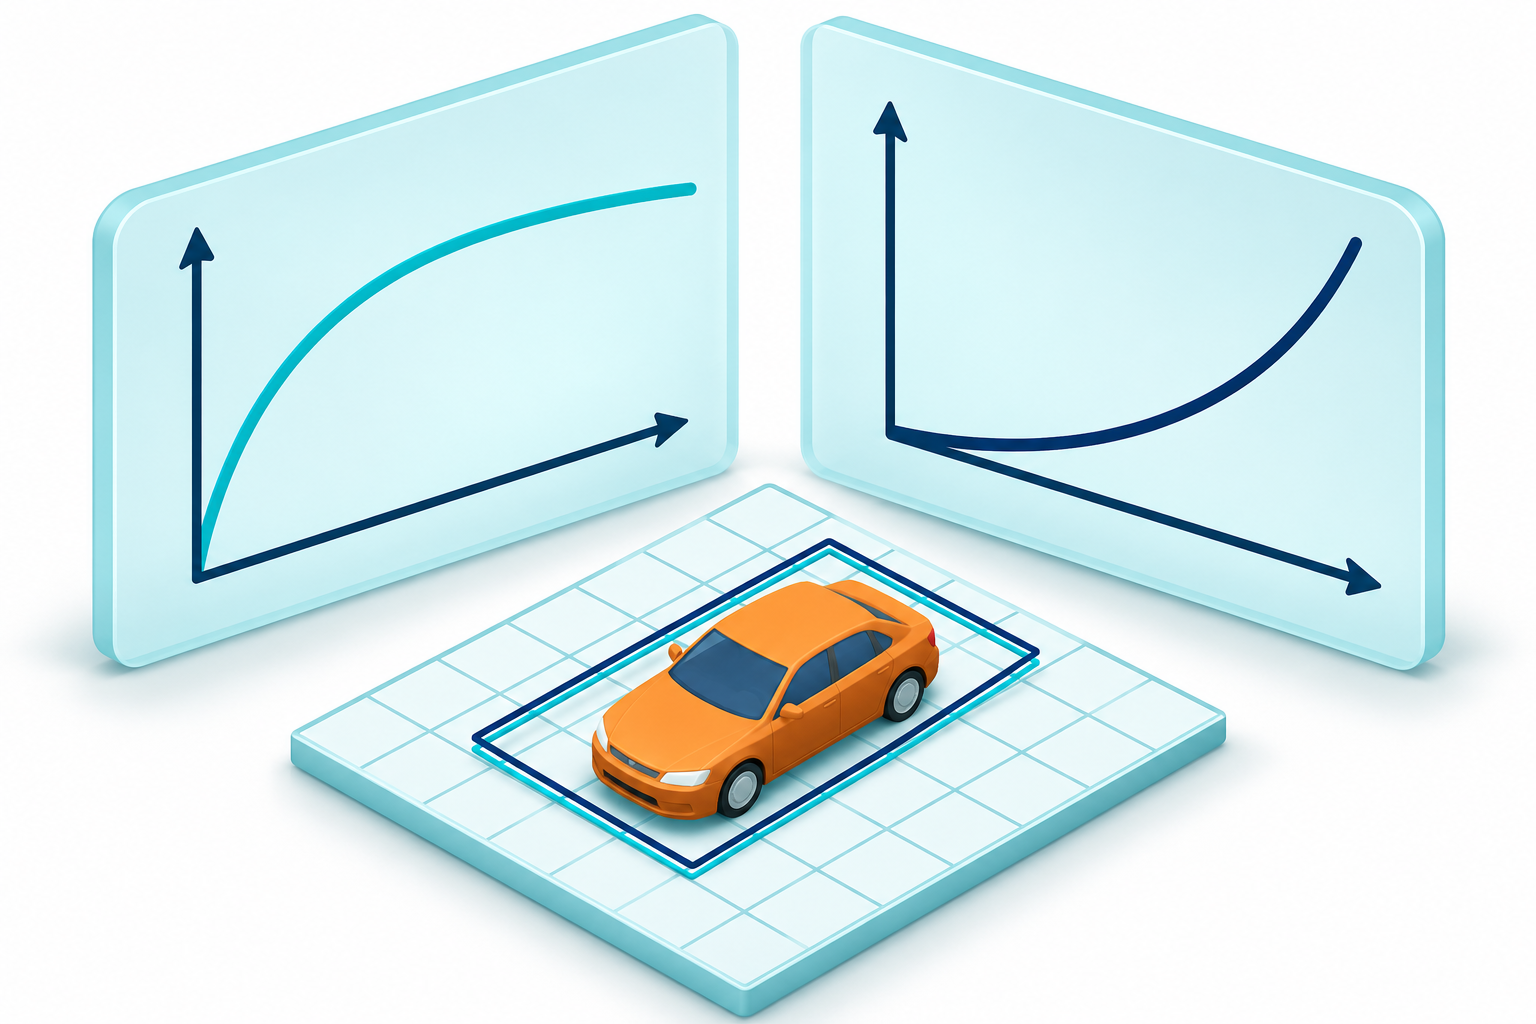
\includegraphics[width=4.0cm,height=2.65cm,keepaspectratio]{assets/illustrations/development/evidence-imagegen-v1.png}};
    \draw[visual arrow] (4.55,3.28) -- (5.25,3.28);
    \draw[visual arrow] (9.55,3.28) -- (10.25,3.28);
    \node[final caption] at (2.4,1.65) {V2X-Sim 2.0};
    \node[final caption] at (7.4,1.65) {Compatible Checkpoints};
    \node[final caption] at (12.4,1.65) {AP + Scaling Curves};
  \end{VisualCanvas}}
  \SlideSource{Source: AI generated illustrations.}
\end{frame}

% src/slides/source/final/sections/01_method_visual.tex

\begin{frame}{How DiscoNet Works}
  \SlideBody{\begin{VisualCanvas}
    \node[final heading] at (2.65,5.35) {Teacher + Student};
    \node[anchor=north,inner sep=0pt] at (2.65,4.9)
      {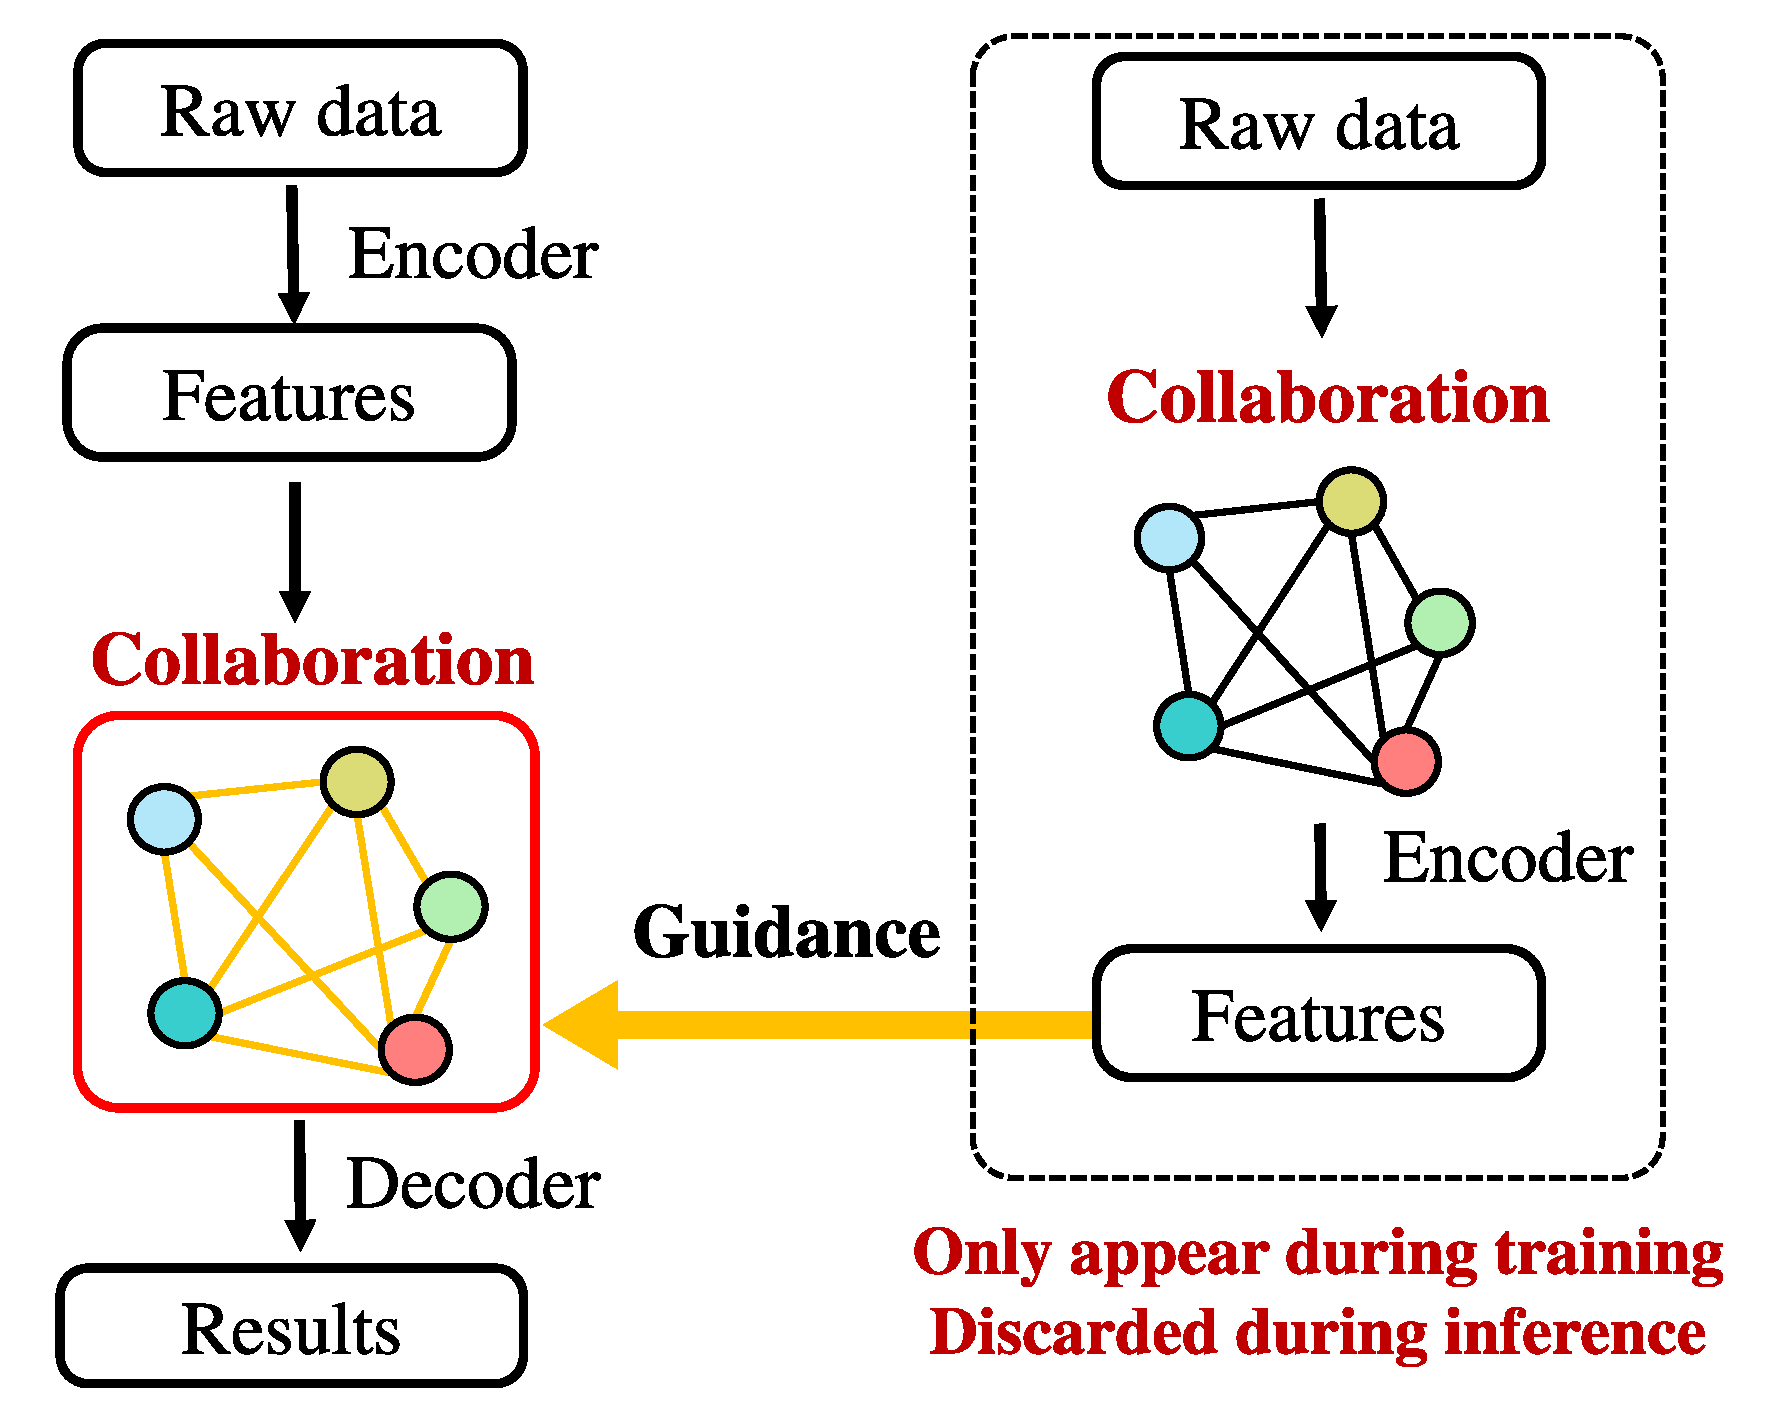
\includegraphics[width=5.4cm,height=4.3cm,keepaspectratio]{assets/papers/disconet/fig1_ours.pdf}};
    \node[final heading] at (10.1,5.35) {Spatial Attention};
    \node[inner sep=0pt] at (10.1,3.6)
      {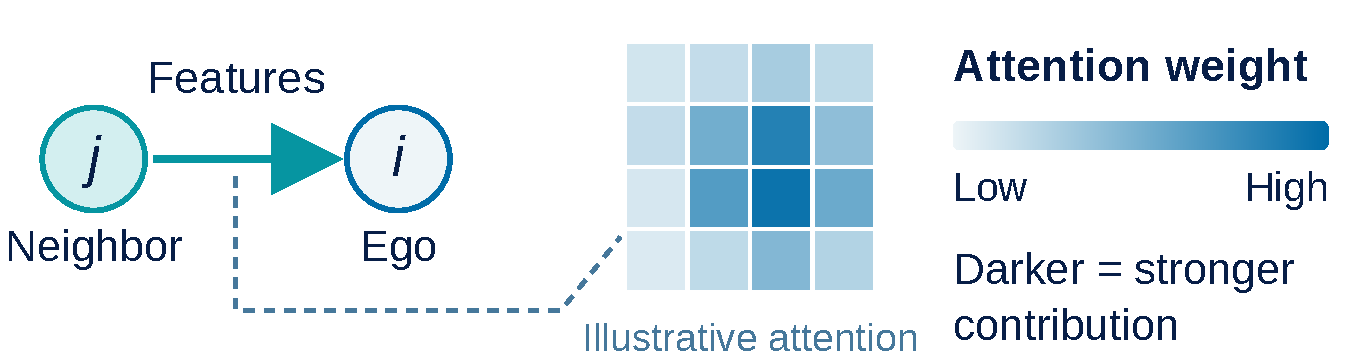
\includegraphics[width=8.65cm]{assets/diagrams/edge-weights.pdf}};
    \node[final caption] at (10.1,1.65) {Share Features\quad Weight by Location};
  \end{VisualCanvas}}
  \SlideSource{Source: Li et al., Fig. 1(c). AI generated attention illustration.}
\end{frame}

% src/slides/source/final/architecture/02_preprocessing.tex

\begin{frame}{LiDAR Preprocessing}
  \SlideBody{\begin{VisualCanvas}
    \node[final heading] at (3.0,5.35) {Point Cloud};
    \node[final heading] at (10.8,5.35) {Occupancy Grid};
    \node[inner sep=0pt] at (3.0,3.1)
      {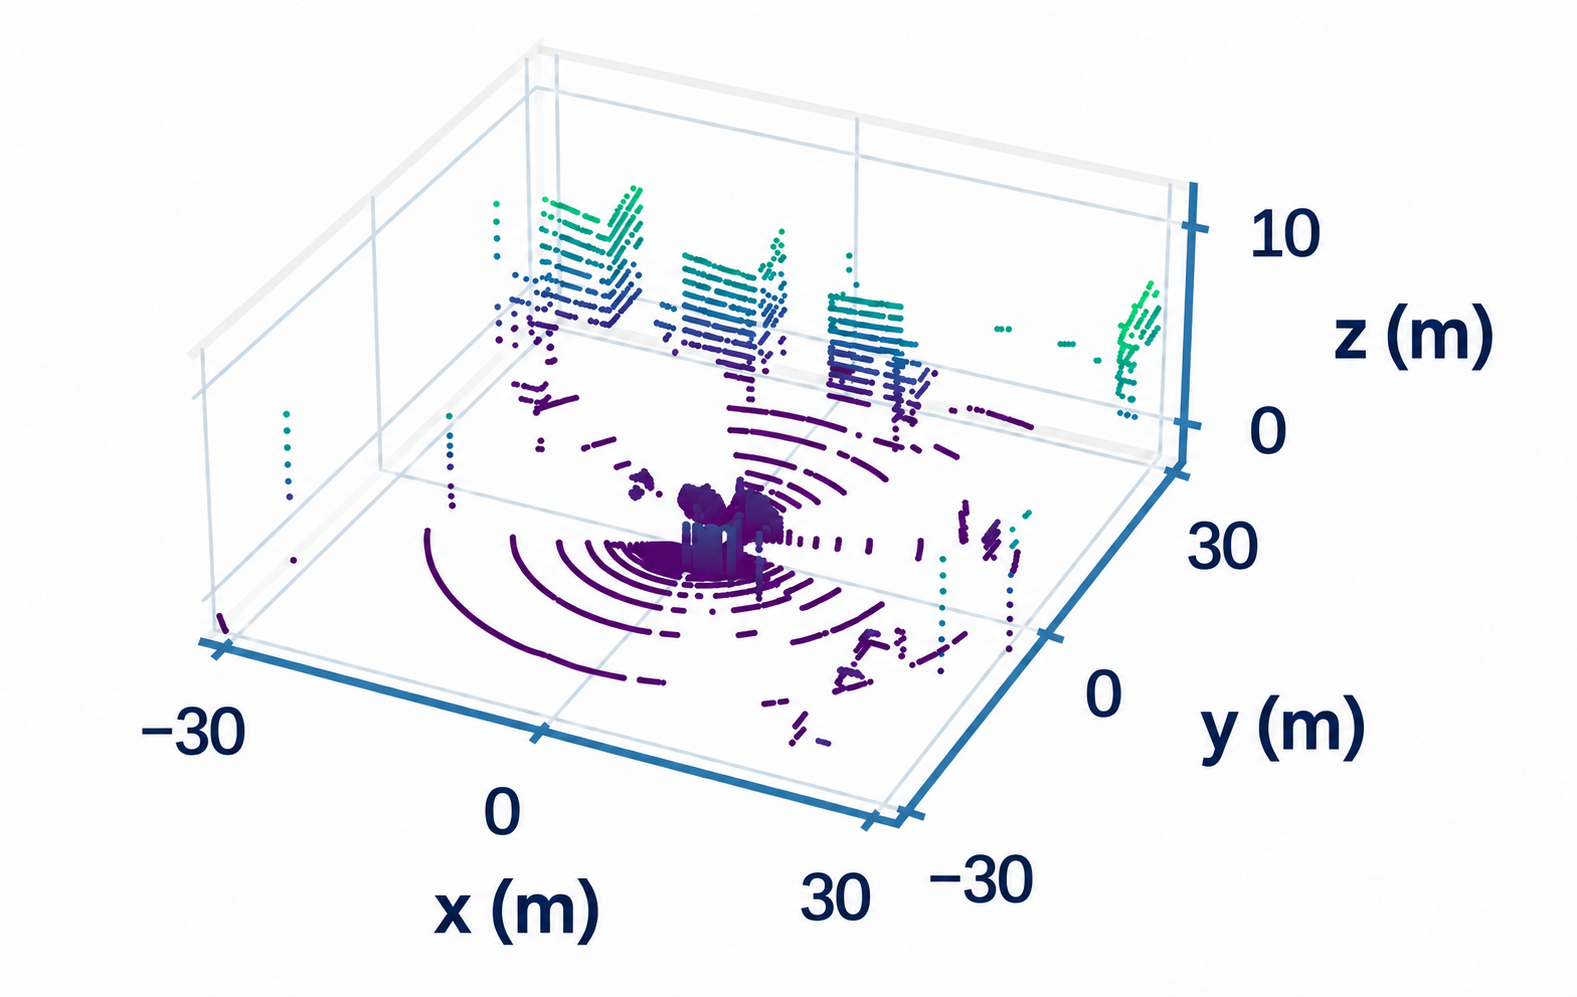
\includegraphics[width=5.8cm,height=4.05cm,keepaspectratio]{assets/architecture/preprocessing/w44_raw_scan-imagegen-v3.png}};
    \node[inner sep=0pt] (occupancy) at (10.8,3.1)
      {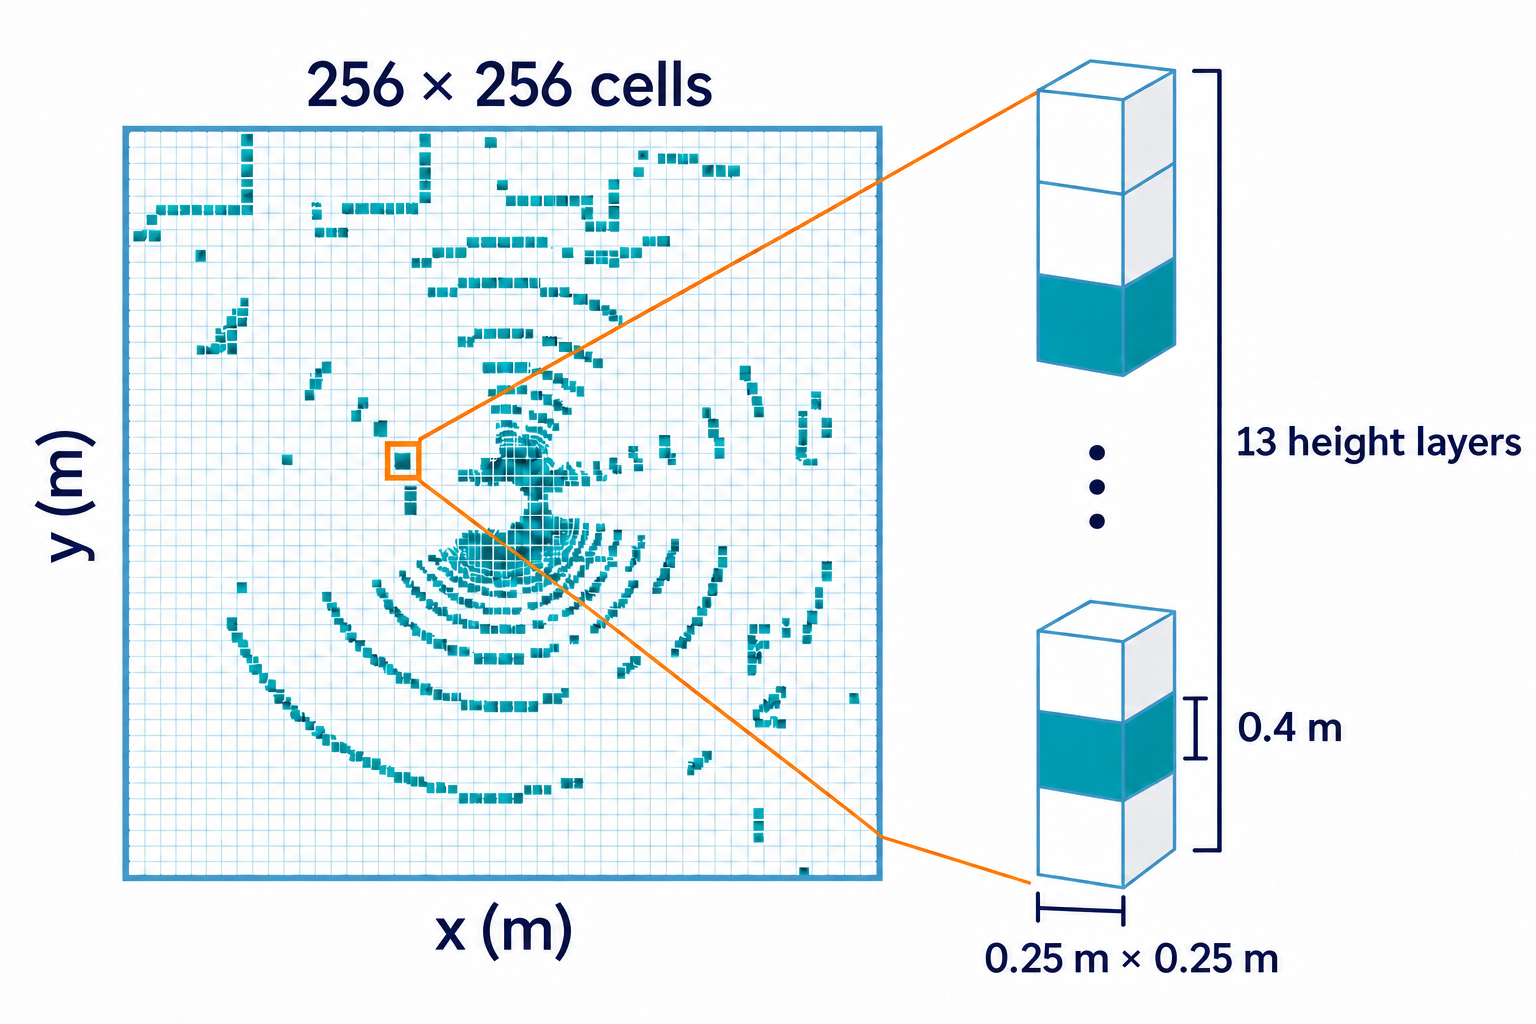
\includegraphics[width=7.2cm,height=4.05cm,keepaspectratio]{assets/architecture/preprocessing/w44_occupancy_layers-imagegen-v3.png}};
    \draw[visual arrow] (6.0,3.15) -- (7.05,3.15);
    \node[final caption,anchor=north]
      at ($(occupancy.south)+(0,-0.20)$) {$256\times256\times13$};
    \node[final caption,text width=14.4cm] at (7.4,0.10)
      {1 = Occupied\qquad 0 = No Retained Return};
  \end{VisualCanvas}}
  \SlideSource{Source: CoPerception voxelization. AI generated illustrations.}
\end{frame}

% src/slides/source/final/architecture/05_encoder_pipeline.tex

\begin{frame}{Encoder Pipeline}
  \SlideBody{%
    \centering
    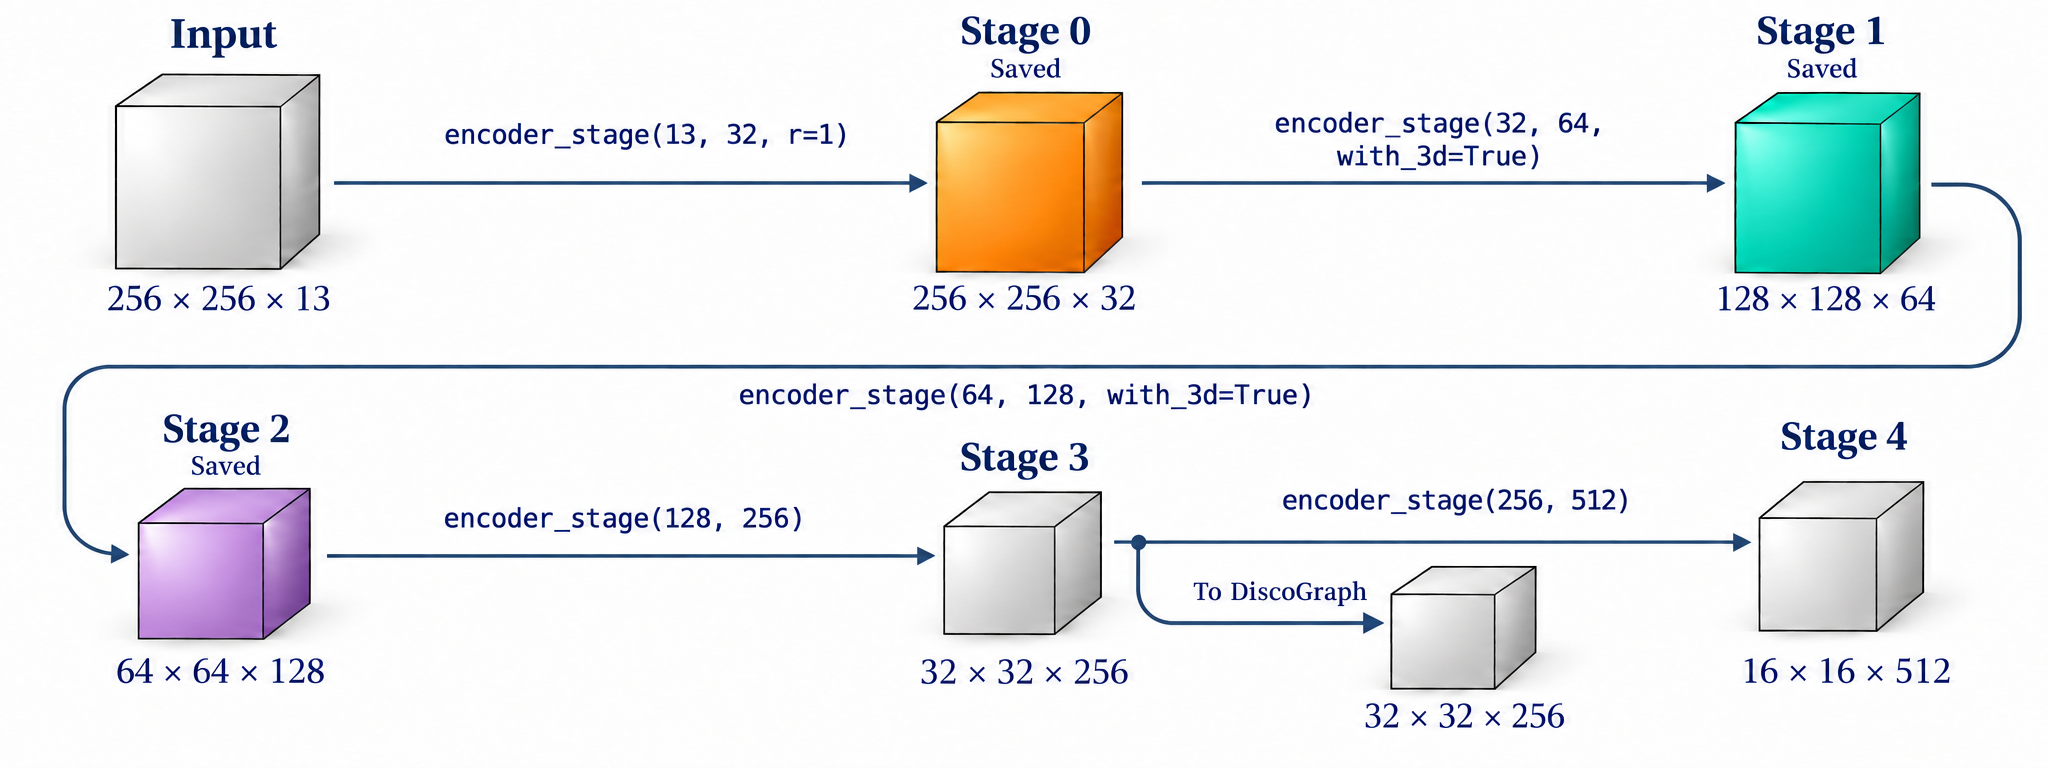
\includegraphics[width=14.65cm,height=5.30cm,keepaspectratio]{assets/architecture/encoder/encoder-stage-pipeline-imagegen-v9.png}\par
    \vspace{0.08cm}
    \FinalTensorLegend
  }
  \SlideSource{Source: CoPerception, \texttt{LidarEncoder} (adapted). AI generated illustration.}
\end{frame}

% src/slides/source/final/architecture/06_discograph.tex

\begin{frame}{DiscoGraph: Spatial Collaboration}
  \SlideBody{\begin{VisualCanvas}
    \node[inner sep=0pt] at (3.6,2.95)
      {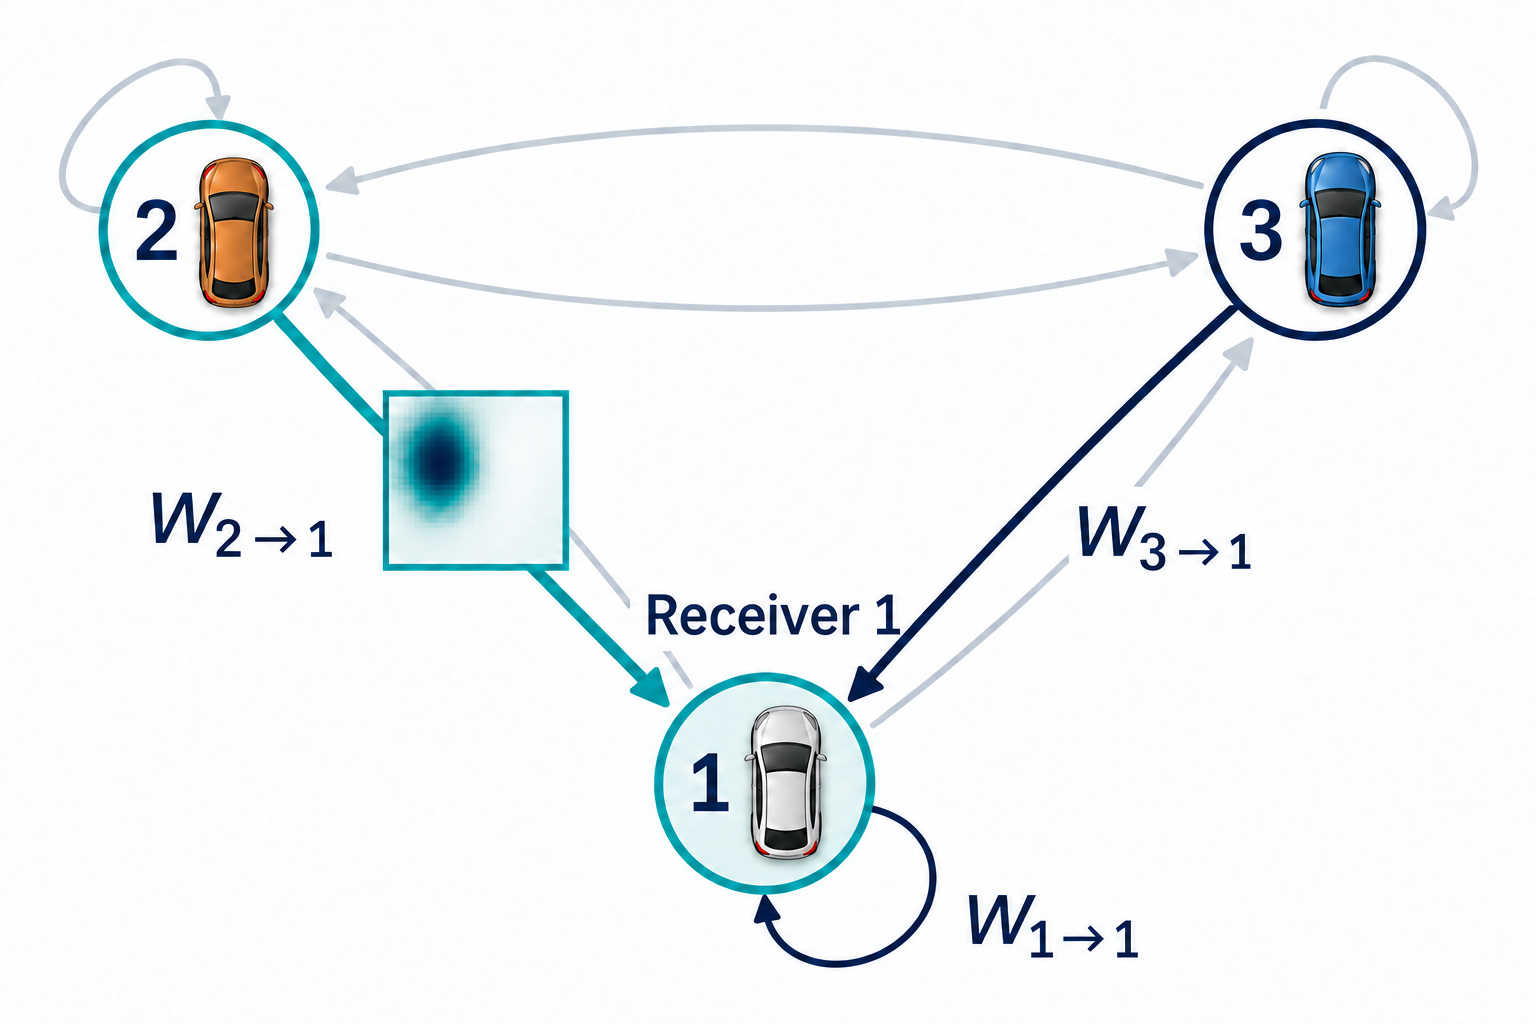
\includegraphics[width=7.15cm,height=3.85cm,keepaspectratio]{assets/architecture/graph/discograph-three-agents-imagegen-v3.png}};
    \node[inner sep=0pt] at (11.2,2.95)
      {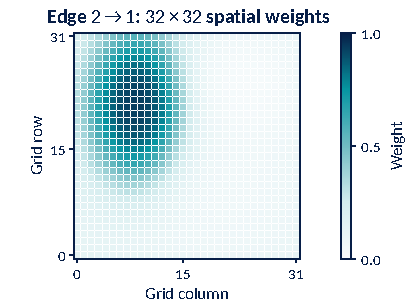
\includegraphics[width=6.85cm,height=3.85cm,keepaspectratio]{assets/architecture/graph/discograph-three-agents-v2-spatial-map.pdf}};
    \VisualTakeaway{$\sum_u w_{u\to v}(r,c)=1$}
  \end{VisualCanvas}}
  \SlideSource{Source: Li et al., Sec. 2.1. AI generated illustrations.}
\end{frame}

% src/slides/source/final/architecture/08_decoder_pipeline.tex

\begin{frame}{Decoder Pipeline}
  \SlideBody{%
    \centering
    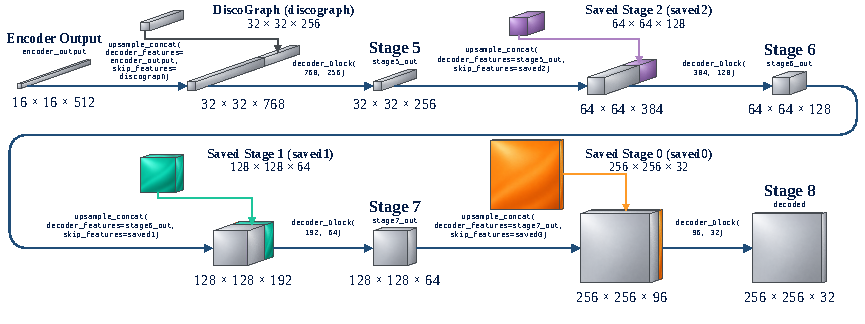
\includegraphics[width=14.65cm,height=5.30cm,keepaspectratio]{assets/architecture/decoder/decoder-stage-pipeline-v6.pdf}\par
    \vspace{0.08cm}
    \FinalTensorLegend
  }
  \SlideSource{Source: CoPerception, \texttt{LidarDecoder} (adapted). AI generated illustration.}
\end{frame}


\section{Evaluation}
% Four original AI-generated scenes illustrate the experiment assumptions.
% Headings and captions use the deck's native typography, not bitmap text.
\begin{frame}{Perfect Communication}
  \SlideBody{%
    \centering
    {\fontsize{11}{13}\selectfont\bfseries\color{MoverDetailBlue}
      \makebox[3.6cm]{Synchronized}%
      \makebox[3.6cm]{Accurate Poses}%
      \makebox[3.6cm]{Zero Delay}%
      \makebox[3.6cm]{No Packet Loss}\par}
    \vspace{0.06cm}
    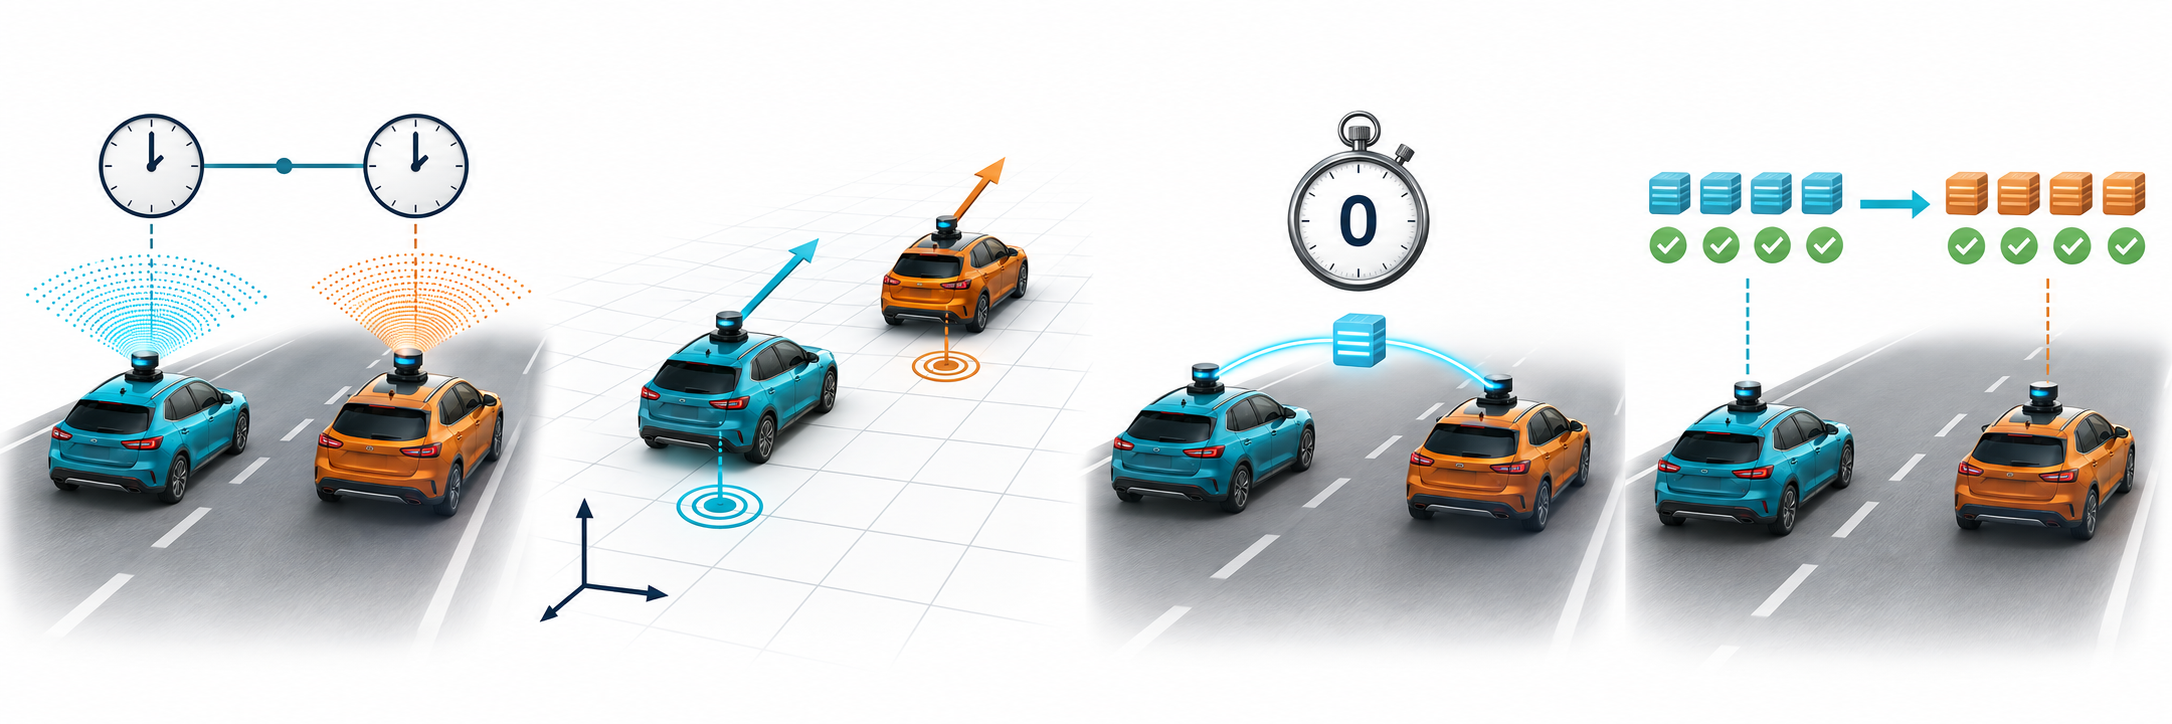
\includegraphics[width=14.4cm,height=4.80cm,keepaspectratio]{assets/illustrations/perfect-communication.png}\par
    \vspace{0.03cm}
    {\fontsize{10.5}{13}\selectfont
      % Zero-size overlays divide the four columns without moving their content.
      \makebox[0pt][l]{\hspace*{3.6cm}\raisebox{-0.05cm}[0pt][0pt]{\textcolor{MoverDetailBlue!40}{\rule{0.60pt}{5.70cm}}}}%
      \makebox[0pt][l]{\hspace*{7.2cm}\raisebox{-0.05cm}[0pt][0pt]{\textcolor{MoverDetailBlue!40}{\rule{0.60pt}{5.70cm}}}}%
      \makebox[0pt][l]{\hspace*{10.8cm}\raisebox{-0.05cm}[0pt][0pt]{\textcolor{MoverDetailBlue!40}{\rule{0.60pt}{5.70cm}}}}%
      \makebox[3.6cm]{Same observation time}%
      \makebox[3.6cm]{Position and heading}%
      \makebox[3.6cm]{0 ms latency}%
      \makebox[3.6cm]{0\% packet loss}\par}
  }
  \SlideSource{AI-generated illustration.}
\end{frame}

% Editable tables from the recorded configuration and the user's reference.
\begin{frame}{Experiment Setup}
  \definecolor{MoverSetupBlueFill}{HTML}{EAF1F6}
  \definecolor{MoverSetupBlueAltFill}{HTML}{D8E5EF}
  \definecolor{MoverSetupGreenFill}{HTML}{E5F2EF}
  \definecolor{MoverSetupGreenAltFill}{HTML}{CCE5DC}
  \SlideBody{\begin{VisualCanvas}
    \node[anchor=west,inner sep=0pt,text=MoverNavy!75,
      font=\fontsize{11}{14}\selectfont] at (0.0,5.35)
      {Configuration of the completed 1,000-frame benchmark};

    \node[anchor=north west,inner sep=0pt,text=MoverNavy] at (0.0,4.60) {%
      \begin{minipage}{7.0cm}
        \fontsize{10}{12.5}\selectfont
        \setlength{\tabcolsep}{0.15cm}
        \renewcommand{\arraystretch}{1.65}
        \begin{tabular}{>{\raggedright\arraybackslash}p{2.15cm} >{\raggedright\arraybackslash}p{4.25cm}}
          \rowcolor{MoverNavy}
          \multicolumn{2}{l}{\color{white}\fontsize{12}{14}\selectfont\textbf{Hardware}} \\
          \rowcolor{MoverSetupBlueFill}
          \textbf{GPU} & NVIDIA GeForce RTX 5060 Ti \\
          \rowcolor{MoverSetupBlueAltFill}
          \textbf{GPU Memory} & 16 GB \\
          \rowcolor{MoverSetupBlueFill}
          \textbf{CPU} & AMD Ryzen 7 5700X \\
          \rowcolor{MoverSetupBlueAltFill}
          \textbf{CPU Cores} & 8 cores / 16 threads \\
          \rowcolor{MoverSetupBlueFill}
          \textbf{System RAM} & 16 GB \\
        \end{tabular}
      \end{minipage}};

    \node[anchor=north west,inner sep=0pt,text=MoverNavy] at (7.8,4.60) {%
      \begin{minipage}{7.0cm}
        \fontsize{10}{12.5}\selectfont
        \setlength{\tabcolsep}{0.15cm}
        \renewcommand{\arraystretch}{1.65}
        \begin{tabular}{>{\raggedright\arraybackslash}p{2.50cm} >{\raggedright\arraybackslash}p{3.90cm}}
          \rowcolor{MoverNavy}
          \multicolumn{2}{l}{\color{white}\fontsize{12}{14}\selectfont\textbf{Software}} \\
          \rowcolor{MoverSetupGreenFill}
          \textbf{OS} & Omarchy (Linux) \\
          \rowcolor{MoverSetupGreenAltFill}
          \textbf{Python} & 3.14.8 \\
          \rowcolor{MoverSetupGreenFill}
          \textbf{PyTorch} & 2.9.1+cu128 \\
          \rowcolor{MoverSetupGreenAltFill}
          \textbf{CUDA Runtime} & 12.8 \\
        \end{tabular}
      \end{minipage}};
  \end{VisualCanvas}}
  \SlideSource{Source: Recorded benchmark configuration, November 3.}
\end{frame}

% Values and vector precision/recall curves are copied from the full test run.
\begin{frame}{Cooperation Improves Detection}
  \SlideBody{\begin{VisualCanvas}
    \node[anchor=north,inner sep=0pt,text=MoverNavy,
      font=\fontsize{11}{13}\selectfont] at (7.4,5.66) {%
      \renewcommand{\arraystretch}{1.00}
      \begin{tabular}{@{}lcc@{}}
        \toprule
        \makebox[6.1cm][l]{\textbf{Condition}} &
        \makebox[3.25cm]{\textbf{AP@0.5 (\%)}} &
        \makebox[3.25cm]{\textbf{AP@0.7 (\%)}} \\
        \midrule
        Own Scan Only & 49.10 & 43.05 \\
        \textbf{Cooperative Perception} & \textbf{70.41} & \textbf{64.82} \\
        \bottomrule
      \end{tabular}};
    \node[inner sep=0pt] at (7.4,2.00)
      {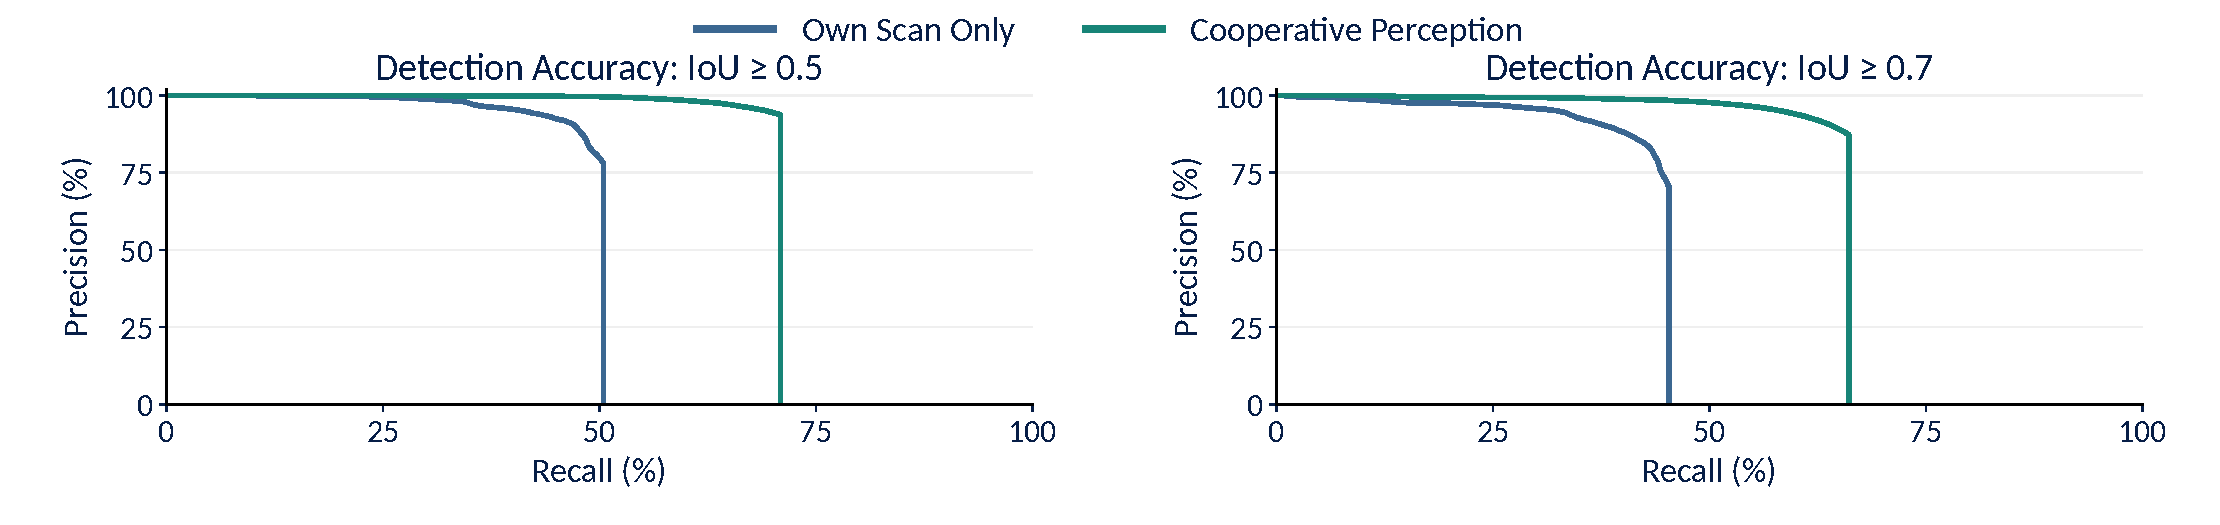
\includegraphics[width=14.4cm,height=3.45cm,keepaspectratio]{assets/experiments/w45-2026-11-04/results-plots-v1.pdf}};
    \node[final caption,font=\bfseries\fontsize{12}{15}\selectfont]
      at (7.4,0.15) {Sharing Adds 21.31 / 21.77 AP Percentage Points};
  \end{VisualCanvas}}
  \SlideSource{Source: Li et al., DiscoNet (method).}
\end{frame}


\section{Results}
\begin{frame}{Original vs. Tree Collaboration}
  \SlideBody{\begin{VisualCanvas}
    \node[final heading,font=\bfseries\fontsize{13}{16}\selectfont]
      at (3.65,5.30) {Original: Complete Graph};
    \node[final heading,font=\bfseries\fontsize{13}{16}\selectfont]
      at (11.10,5.30) {Tree: Maximum Spanning Tree};

    \foreach \Agent in {1,...,5} {
      \pgfmathsetmacro{\Angle}{90+360*(\Agent-1)/5}
      \coordinate (full-node-\Agent) at
        ({3.65+1.45*cos(\Angle)},{2.90+1.45*sin(\Angle)});
      \coordinate (tree-node-\Agent) at
        ({11.10+1.45*cos(\Angle)},{2.90+1.45*sin(\Angle)});
    }
    \foreach \Sender in {1,...,5} {
      \foreach \Receiver in {1,...,5} {
        \ifnum\Sender<\Receiver
          \draw[{Stealth[length=1.1mm]}-{Stealth[length=1.1mm]},
            draw=MoverNavy!35,line width=0.55pt,shorten <=4pt,shorten >=4pt]
            (full-node-\Sender) -- (full-node-\Receiver);
        \fi
      }
    }
    % Saved n=5 preflight tree; logical node IDs are shown one-based.
\draw[{Stealth[length=1.1mm]}-{Stealth[length=1.1mm]},draw=MoverCyan,line width=1.0pt,shorten <=4pt,shorten >=4pt] (tree-node-3) -- (tree-node-4);
\draw[{Stealth[length=1.1mm]}-{Stealth[length=1.1mm]},draw=MoverCyan,line width=1.0pt,shorten <=4pt,shorten >=4pt] (tree-node-1) -- (tree-node-2);
\draw[{Stealth[length=1.1mm]}-{Stealth[length=1.1mm]},draw=MoverCyan,line width=1.0pt,shorten <=4pt,shorten >=4pt] (tree-node-2) -- (tree-node-3);
\draw[{Stealth[length=1.1mm]}-{Stealth[length=1.1mm]},draw=MoverCyan,line width=1.0pt,shorten <=4pt,shorten >=4pt] (tree-node-4) -- (tree-node-5);

    \foreach \Agent in {1,...,5} {
      \foreach \Prefix in {full,tree} {
        \node[circle,fill=MoverNavy,draw=MoverCyan,line width=0.8pt,
          minimum size=0.36cm,inner sep=0pt,text=white,
          font=\bfseries\fontsize{8}{9}\selectfont]
          at (\Prefix-node-\Agent) {\Agent};
      }
    }
    \draw[visual arrow] (5.50,2.90) -- (9.25,2.90);
    \node[final caption,font=\fontsize{10}{13}\selectfont] at (7.4,2.38)
      {Kruskal Selection};
    \node[final caption] at (3.65,1.00)
      {$n^2$ Directed Edges};
    \node[final caption] at (11.10,1.00)
      {$3n-2$ Directed Edges};
  \end{VisualCanvas}}
  \SlideSource{Source: Own elaboration.}
\end{frame}

% Generated from tree-comparison.csv by generate_table.py.
\long\def\TreeStudyTableRows{%
\rowcolor{TreeDistinctLight}
1 & 7.82 & 7.86 & 48.91 & 48.91 & 45.54 & 45.54 \\
\rowcolor{TreeDistinctAlt}
2 & 13.34 & 13.25 & 60.94 & 60.94 & 53.67 & 53.67 \\
\rowcolor{TreeDistinctLight}
3 & 21.99 & 21.41 & 66.52 & 60.17 & 58.71 & 52.34 \\
\rowcolor{TreeDistinctAlt}
4 & 31.39 & 29.38 & 70.80 & 58.06 & 63.39 & 50.37 \\
\rowcolor{TreeDistinctLight}
5 & 41.57 & 36.54 & 74.46 & 62.65 & 67.53 & 53.66 \\
\rowcolor{TreeReplayAlt}
6 & 52.43 & 43.63 & 73.54 & 57.71 & 66.61 & 50.69 \\
\rowcolor{TreeReplayLight}
7 & 66.67 & 52.89 & 73.93 & 57.87 & 66.70 & 50.57 \\
\rowcolor{TreeReplayAlt}
8 & 79.83 & 60.47 & 73.80 & 59.16 & 66.90 & 52.01 \\
\rowcolor{TreeReplayLight}
9 & 92.07 & 67.48 & 74.50 & 61.56 & 67.06 & 53.33 \\
\rowcolor{TreeReplayAlt}
10 & 102.80 & 70.12 & 74.46 & 61.72 & 67.53 & 53.66 \\
\rowcolor{TreeReplayLight}
11 & 118.76 & 76.93 & 74.00 & 58.57 & 67.05 & 50.44 \\
\rowcolor{TreeReplayAlt}
12 & 133.49 & 82.84 & 74.17 & 58.77 & 67.20 & 50.72 \\
\rowcolor{TreeReplayLight}
13 & 147.97 & 86.52 & 74.36 & 59.50 & 67.18 & 51.61 \\
\rowcolor{TreeReplayAlt}
14 & 165.79 & 92.73 & 74.90 & 60.93 & 67.50 & 52.75 \\
\rowcolor{TreeReplayLight}
\textbf{15} & \textbf{185.05} & \textbf{99.25} & \textbf{74.46} & \textbf{60.48} & \textbf{67.53} & \textbf{52.45} \\
}

\begin{frame}{Runtime and Detection AP}
  \definecolor{TreeDistinctLight}{HTML}{EAF1F6}
  \definecolor{TreeDistinctAlt}{HTML}{D8E5EF}
  \definecolor{TreeReplayLight}{HTML}{E5F2EF}
  \definecolor{TreeReplayAlt}{HTML}{CCE5DC}
  \SlideBody{\begin{VisualCanvas}
    \node[anchor=north,inner sep=0pt,text=MoverNavy,
      font=\fontsize{9}{10.5}\selectfont] at (7.4,5.58) {%
      \setlength{\tabcolsep}{0.06cm}
      \setlength{\arrayrulewidth}{0.5pt}
      \arrayrulecolor{MoverNavy!35}
      \renewcommand{\arraystretch}{0.78}
      \begin{tabular}{>{\centering\arraybackslash}p{0.60cm}|*{2}{>{\centering\arraybackslash}p{2.20cm}}|*{2}{>{\centering\arraybackslash}p{2.20cm}}|*{2}{>{\centering\arraybackslash}p{2.20cm}}}
        \rowcolor{MoverNavy}
        \color{white}\textbf{$n$} &
        \color{white}\shortstack{\textbf{Original}\\\textbf{Median (ms)}} &
        \color{white}\shortstack{\textbf{Tree}\\\textbf{Median (ms)}} &
        \color{white}\shortstack{\textbf{Original}\\\textbf{AP@0.5 (\%)}} &
        \color{white}\shortstack{\textbf{Tree}\\\textbf{AP@0.5 (\%)}} &
        \color{white}\shortstack{\textbf{Original}\\\textbf{AP@0.7 (\%)}} &
        \color{white}\shortstack{\textbf{Tree}\\\textbf{AP@0.7 (\%)}} \\
        \TreeStudyTableRows
      \end{tabular}};
  \end{VisualCanvas}}
  \SlideSource{Source: Own elaboration.}
\end{frame}

% Generated from the n=15 row. AP changes are percentage points.
\def\TreeStudyTimeReduction{46.4}
\def\TreeStudyOriginalTime{185.05}
\def\TreeStudyTreeTime{99.25}
\def\TreeStudyOriginalAPFifty{74.46}
\def\TreeStudyTreeAPFifty{60.48}
\def\TreeStudyOriginalAPSeventy{67.53}
\def\TreeStudyTreeAPSeventy{52.45}
\def\TreeStudyAPFiftyDelta{-13.98}
\def\TreeStudyAPSeventyDelta{-15.08}

\begin{frame}{Runtime and Accuracy Trade-Off}
  \SlideBody{\begin{VisualCanvas}
    \node[final caption,font=\fontsize{12}{15}\selectfont] at (7.4,5.35)
      {At $n=15$\quad Original $\rightarrow$ Tree};
    \node[final heading,font=\bfseries\fontsize{13}{16}\selectfont] at (2.4,4.55) {Inference Time};
    \node[final heading,font=\bfseries\fontsize{13}{16}\selectfont] at (7.4,4.55) {AP@0.5};
    \node[final heading,font=\bfseries\fontsize{13}{16}\selectfont] at (12.4,4.55) {AP@0.7};
    \foreach \Col in {4.9,9.9} {\draw[draw=MoverNavy!20] (\Col,1.55) -- (\Col,4.80);}
    \node[final statement,font=\bfseries\fontsize{32}{38}\selectfont]
      at (2.4,3.45) {\TreeStudyTimeReduction\%};
    \node[final statement,font=\bfseries\fontsize{32}{38}\selectfont]
      at (7.4,3.45) {\TreeStudyAPFiftyDelta};
    \node[final statement,font=\bfseries\fontsize{32}{38}\selectfont]
      at (12.4,3.45) {\TreeStudyAPSeventyDelta};
    \node[final caption,font=\fontsize{11}{14}\selectfont] at (2.4,2.65) {Less Inference Time};
    \node[final caption,font=\fontsize{11}{14}\selectfont] at (7.4,2.65) {Percentage Points};
    \node[final caption,font=\fontsize{11}{14}\selectfont] at (12.4,2.65) {Percentage Points};
    \node[final caption,font=\fontsize{11}{14}\selectfont] at (2.4,1.90)
      {\TreeStudyOriginalTime\ $\rightarrow$ \TreeStudyTreeTime\ ms};
    \node[final caption,font=\fontsize{11}{14}\selectfont] at (7.4,1.90)
      {\TreeStudyOriginalAPFifty\% $\rightarrow$ \TreeStudyTreeAPFifty\%};
    \node[final caption,font=\fontsize{11}{14}\selectfont] at (12.4,1.90)
      {\TreeStudyOriginalAPSeventy\% $\rightarrow$ \TreeStudyTreeAPSeventy\%};
    \node[final caption,font=\bfseries\fontsize{12}{15}\selectfont] at (7.4,1.08)
      {Lower Runtime Comes with Lower Detection AP};
  \end{VisualCanvas}}
  \SlideSource{Source: Own elaboration.}
\end{frame}

\MoverThanksSlide

\appendix
\FinalAppendixtrue
% Supplement to the talk delivered on November 5, 2026.
\section{Appendix}

\begin{frame}[label=appendix-contents]{Appendix Contents}
  \SlideBody{%
    \vspace{0.30cm}
    \renewcommand{\arraystretch}{1.65}
\begin{tabular}{@{}p{0.65cm}p{10.5cm}r@{}}
\textbf{A} & \hyperlink{appendix-architecture}{Architecture and Implementation} & \hyperlink{appendix-architecture}{A3--A26} \\
\textbf{B} & \hyperlink{appendix-evaluation}{Evaluation and Reproduction} & \hyperlink{appendix-evaluation}{A27--A37} \\
\textbf{C} & \hyperlink{appendix-convolutions}{Conv2D and Conv3D} & \hyperlink{appendix-convolutions}{A38--A58} \\
\textbf{D} & \hyperlink{appendix-experiments}{Complete Experiment Record} & \hyperlink{appendix-experiments}{A59--A79} \\
\textbf{E} & \hyperlink{appendix-image-generation}{Image Generation Example} & \hyperlink{appendix-image-generation}{A80--A83} \\
\end{tabular}
\par
  }
\end{frame}

% Each appendix group has an explicit divider with its own description.
\AtBeginSection[]{}
% Generated by final/appendix/generate.py; edit sources.json.

\FinalAppendixDivider{A}{Architecture and Implementation}{architecture}{Voxelization, reusable blocks, encoder code, spatial alignment, attention, fusion, and decoding.}
\FinalWeeklyAppendixPage{7}{LiDAR Preprocessing}
\FinalWeeklyAppendixPage{8}{Voxelization}
\FinalWeeklyAppendixPage{10}{Normalization and Activation}
\FinalWeeklyAppendixPage{11}{2D Unit}
\FinalWeeklyAppendixPage{12}{2D Unit: Variants}
\FinalWeeklyAppendixPage{13}{2D Pointwise Unit}
\FinalWeeklyAppendixPage{14}{Decoder Block}
\FinalWeeklyAppendixPage{15}{3D Convolution}
\FinalWeeklyAppendixPage{16}{Encoder Stage}
\FinalWeeklyAppendixPage{17}{Upsample and Concat}
\FinalWeeklyAppendixPage{18}{Decoder Stage}
\FinalWeeklyAppendixPage{20}{Encoder Pipeline}
\FinalWeeklyAppendixPage{21}{Encoder Code}
\FinalWeeklyAppendixPage{23}{DiscoGraph}
\FinalWeeklyAppendixPage{24}{DiscoGraph: Feature Alignment}
\FinalWeeklyAppendixPage{25}{DiscoGraph: Rotate and Translate}
\FinalWeeklyAppendixPage{26}{DiscoGraph: Alignment in PyTorch}
\FinalWeeklyAppendixPage{27}{DiscoGraph: Pair the Features}
\FinalWeeklyAppendixPage{28}{DiscoGraph: Edge Scores}
\FinalWeeklyAppendixPage{29}{DiscoGraph: Spatial Weights}
\FinalWeeklyAppendixPage{30}{DiscoGraph: Weighted Features}
\FinalWeeklyAppendixPage{31}{DiscoGraph: Fused Features}
\FinalWeeklyAppendixPage{33}{Decoder Pipeline}

\FinalAppendixDivider{B}{Evaluation and Reproduction}{evaluation}{IoU, confidence scores, precision and recall, AP, dataset statistics, camera views, and benchmark results.}
\FinalWeeklyAppendixPage{35}{Intersection over Union (IoU)}
\FinalWeeklyAppendixPage{36}{IoU: Matching Thresholds}
\FinalWeeklyAppendixPage{37}{DiscoNet Confidence Scores}
\FinalWeeklyAppendixPage{38}{Precision, Recall, and AP}
\FinalWeeklyAppendixPage{39}{V2X-Sim 2.0: Dataset Analysis}
\FinalWeeklyAppendixPage{40}{V2X-Sim 2.0: Car Detections}
\FinalWeeklyAppendixPage{41}{V2X-Sim 2.0: Camera Views}
\FinalWeeklyAppendixPage{42}{Experiment Setup}
\FinalWeeklyAppendixPage{43}{V2X-Sim 2.0: Reproduced Results}
\FinalWeeklyAppendixPage{44}{V2X-Sim 2.0: Runtime Scaling}

\FinalAppendixDivider{C}{Conv2D and Conv3D}{convolutions}{The complete numerical walkthrough: input tensor, kernels, and every spatial and temporal sliding window.}
\FinalWeeklyAppendixPage{50}{Initial Tensor}
\FinalWeeklyAppendixPage{51}{Kernels}
\FinalWeeklyAppendixPage{52}{Conv2D: Sliding Window}
\FinalWeeklyAppendixPage{53}{Conv2D: Sliding Window}
\FinalWeeklyAppendixPage{54}{Conv2D: Sliding Window}
\FinalWeeklyAppendixPage{55}{Conv2D: Sliding Window}
\FinalWeeklyAppendixPage{56}{Conv2D: Sliding Window}
\FinalWeeklyAppendixPage{57}{Conv2D: Sliding Window}
\FinalWeeklyAppendixPage{58}{Conv3D: Sliding Window}
\FinalWeeklyAppendixPage{59}{Conv3D: Sliding Window}
\FinalWeeklyAppendixPage{60}{Conv3D: Sliding Window}
\FinalWeeklyAppendixPage{61}{Conv3D: Sliding Window}
\FinalWeeklyAppendixPage{62}{Conv3D: Sliding Window}
\FinalWeeklyAppendixPage{63}{Conv3D: Sliding Window}
\FinalWeeklyAppendixPage{64}{Conv3D: Sliding Window}
\FinalWeeklyAppendixPage{65}{Conv3D: Sliding Window}
\FinalWeeklyAppendixPage{66}{Conv3D: Sliding Window}
\FinalWeeklyAppendixPage{67}{Conv3D: Sliding Window}
\FinalWeeklyAppendixPage{68}{Conv3D: Sliding Window}
\FinalWeeklyAppendixPage{69}{Conv3D: Sliding Window}

\FinalAppendixDivider{D}{Complete Experiment Record}{experiments}{All 20 report pages: recorded examples, training and test protocol, losses, runtime scaling, and Original/Tree results.}
\FinalExperimentAppendixPage{1}{DiscoNet: Our First Experiment}
\FinalExperimentAppendixPage{2}{Example 1: Reference and Predicted Car Boxes}
\FinalExperimentAppendixPage{3}{Example 1: Camera Views}
\FinalExperimentAppendixPage{4}{V2X-Sim 2.0: Dataset Overview}
\FinalExperimentAppendixPage{5}{Authors' Training Setup and Dataset Splits}
\FinalExperimentAppendixPage{6}{Dataset Statistics by Partition and Vehicle Inputs}
\FinalExperimentAppendixPage{7}{Experiment Setup: Hardware and Software}
\FinalExperimentAppendixPage{8}{Experiment Procedure, Metrics, and Running Time}
\FinalExperimentAppendixPage{9}{Original Test Split: Loss and Detection Accuracy}
\FinalExperimentAppendixPage{10}{How DiscoNet Computes Confidence Scores}
\FinalExperimentAppendixPage{11}{How Precision–Recall Curves and AP Are Computed}
\FinalExperimentAppendixPage{12}{Original Test Split: Accuracy and Loss Plots}
\FinalExperimentAppendixPage{13}{Custom Experiments}
\FinalExperimentAppendixPage{14}{Custom Experiment 1: V2X-Sim Inputs and Replay}
\FinalExperimentAppendixPage{15}{Custom Experiment 1: Measuring Runtime}
\FinalExperimentAppendixPage{16}{Custom Experiment 1: Runtime Results for n = 1–10}
\FinalExperimentAppendixPage{17}{Custom Experiment 1: Runtime Results for n = 11–20}
\FinalExperimentAppendixPage{18}{Custom Experiment 1: Runtime Versus Model Input Count}
\FinalExperimentAppendixPage{19}{Custom Experiment 2: Coarse Attention and Kruskal Fusion}
\FinalExperimentAppendixPage{20}{Custom Experiment 2: Runtime and Detection AP}

\FinalAppendixDivider{E}{Image Generation Example}{image-generation}{Codex CLI, the generation prompt, and the result.}
\begin{frame}{Simple Workflow}
  \SlideBody{%
    {\fontsize{13}{17}\selectfont
    \textbf{I used OpenAI Codex CLI with my ChatGPT account.}\par}
    \vspace{0.40cm}
    {\fontsize{12}{16}\selectfont
    \textbf{Get Access:} Use a
    \href{https://learn.chatgpt.com/docs/pricing}{ChatGPT Plus or Pro subscription},
    install \href{https://learn.chatgpt.com/docs/codex/cli}{Codex CLI},
    and choose \textbf{Sign in with ChatGPT}.\par
    \vspace{0.45cm}
    \textbf{1.} Describe the image in a prompt.\par
    \vspace{0.22cm}
    \textbf{2.} Put the generated image in the slide.\par}
  }
  \SlideSource{OpenAI documentation:
    \href{https://learn.chatgpt.com/docs/codex/cli}{Codex CLI} and
    \href{https://learn.chatgpt.com/docs/pricing}{ChatGPT subscriptions}.}
\end{frame}

\begin{frame}{Prompt: Generate the Image}
  \SlideBody{%
    \vspace{0.12cm}
    {\fontsize{10.5}{13.2}\selectfont
    \input{assets/illustrations/prompt-trials-2026-11-09/first-prompt.generated}\par}
  }
  \SlideSource{Tested reconstruction; November 9, 2026.}
\end{frame}

\begin{frame}{Generated Result}
  \SlideBody{\centering
    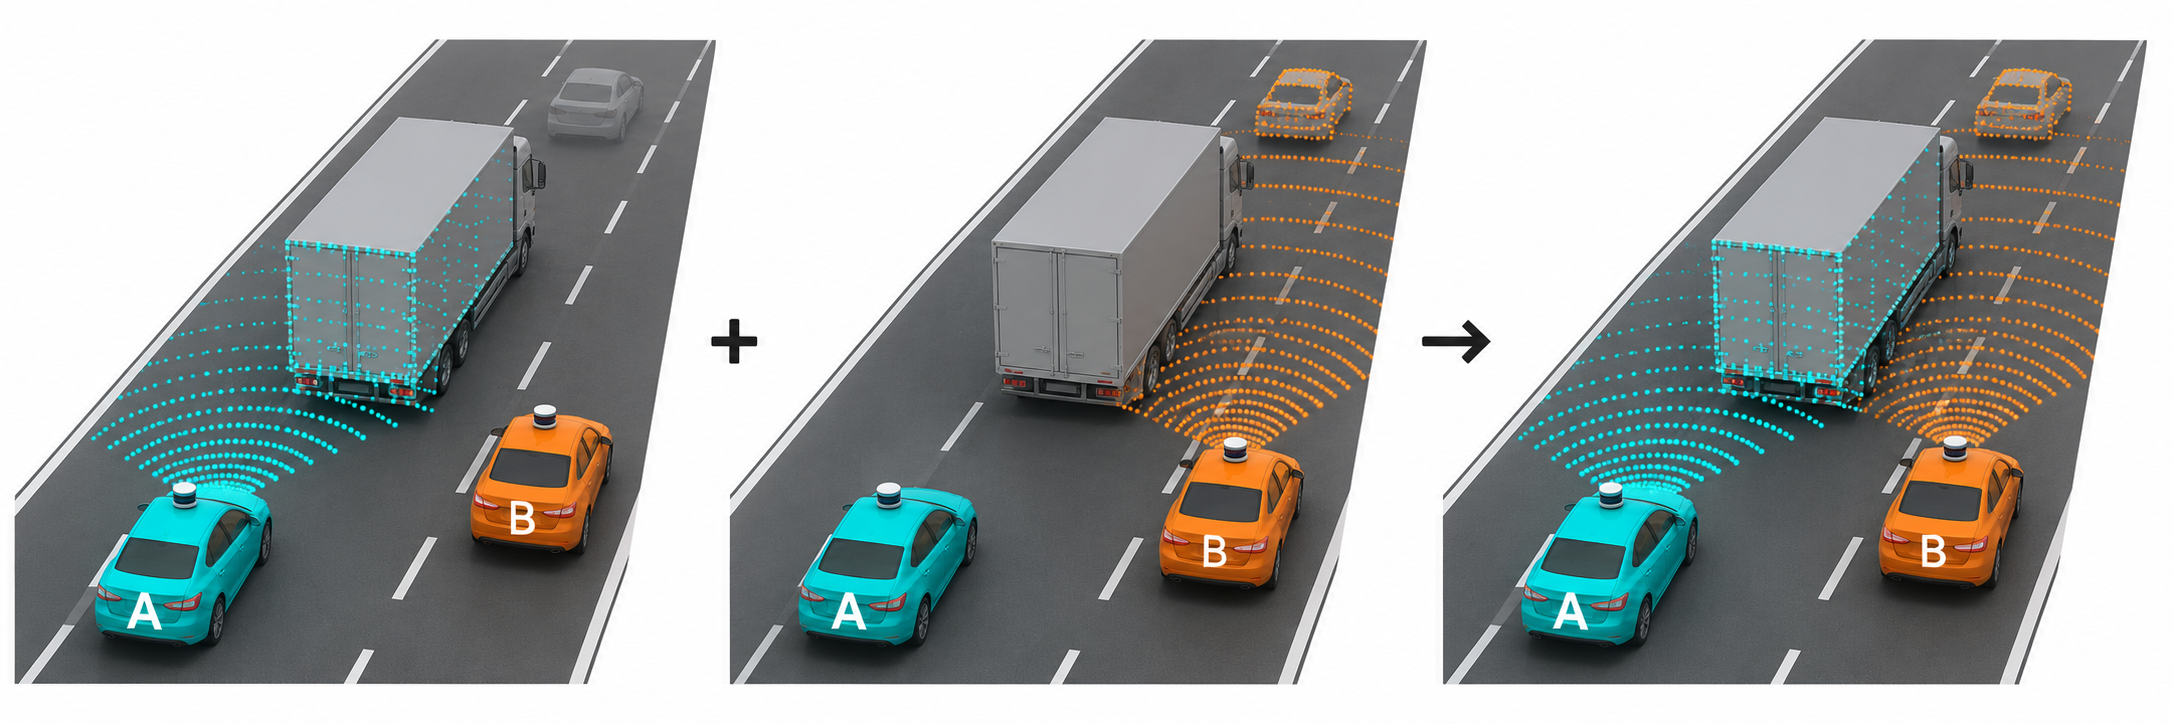
\includegraphics[width=14.65cm,height=4.90cm,keepaspectratio]
      {illustrations/prompt-trials-2026-11-09/layout-preservation-initial.png}\par
    \vspace{0.16cm}
    {\fontsize{11}{14}\selectfont Result from the prompt.\par}
  }
  \SlideSource{Source: AI generated illustration.}
\end{frame}




\end{document}
